
% ----------------------------------------------------------------
% AMS-LaTeX Paper ************************************************
% **** -----------------------------------------------------------
\documentclass[11pt]{amsart}
\usepackage{graphicx, mathabx, amssymb,amsfonts,amsmath,amsthm,newlfont,mathtools}
\usepackage{epsfig,url}
\usepackage[usenames,dvipsnames]{color}
\usepackage{enumerate}
\usepackage[colorlinks=true,linkcolor=red,citecolor=blue]{hyperref}
\usepackage{color}
\usepackage{stmaryrd}         % Crochet double barre (entiers)

% !TEX root = ../Poissons.tex




%Clever ref
\usepackage[noabbrev,capitalize]{cleveref}
\usepackage[all,2cell]{xy} \UseAllTwocells \SilentMatrices

%MARGINS

\setlength{\textwidth}{\paperwidth}
\addtolength{\textwidth}{-2.5in}
\calclayout


% ----------------------------------------------------------------
\vfuzz2pt % Don't report over-full v-boxes if over-edge is small
\hfuzz2pt % Don't report over-full h-boxes if over-edge is small
% THEOREMS -------------------------------------------------------
\newtheorem{thm}{Theorem}[section]
\newtheorem{corollary}[thm]{Corollary}
\newtheorem{lemma}[thm]{Lemma}
\newtheorem{construction}[thm]{Construction}
\newtheorem{proposition}[thm]{Proposition}
\newtheorem{Questions}[thm]{Questions}
\theoremstyle{definition}
\newtheorem{definition}[thm]{Definition}

\newtheorem{conjectue}{Conjecture} 
\newtheorem{QQ}{Question} 
\newtheorem{prob}{Problem}
\newtheorem{ex}[thm]{Examples}
\newtheorem{example}[thm]{Example}
\newtheorem{policy}{Policy}
\theoremstyle{remark}
\newtheorem{rem}[thm]{Remark}
\newtheorem{caveat}[thm]{Caveat}
\numberwithin{equation}{section}
% MATH -----------------------------------------------------------
\newcommand{\norm}[1]{\left\Vert#1\right\Vert}
\newcommand{\abs}[1]{\left\vert#1\right\vert}
\newcommand{\set}[1]{\left\{#1\right\}}

\newcommand{\To}{\longrightarrow}
\newcommand*{\Longhookrightarrow}{\ensuremath{\lhook\joinrel\relbar\joinrel\rightarrow}}
\newcommand{\Z}{\mathbb Z}
\newcommand{\Q}{\mathbb Q}
\newcommand{\C}{\mathbb C}
\newcommand{\Ok}{\mathcal O}
\newcommand{\ai}{\mathfrak{a}}
\newcommand{\bi}{\mathfrak{b}}
\newcommand{\R}{\mathbb R}
\newcommand{\N}{\mathbb N}
\newcommand{\AM}{A}
\newcommand{\xx}{\mathsf{x}}
\newcommand{\eqv}{\mathrm{ev}}
\font \rus= wncyr10
\newcommand{\sha}{\, \hbox{\rus x} \,}

\newcommand{\Lie}{\mathrm{Lie}}

\newcommand{\GC}{\mathcal{GC}}
\newcommand{\q}{/\!/}

\newcommand{\tr}{\mathrm{tr}}
\newcommand{\id}{\mathrm{id}}

\newcommand{\can}{\mathrm{can}}

\newcommand{\mm}{\mathfrak{m}}

\newcommand{\GL}{\mathrm{GL}}
\newcommand{\LP}{L}
\newcommand{\FL}{F\!L}
\newcommand{\mc}{\mu}

%Important sets 
\newcommand{\EC}{\mathcal{E}} %essential complimentary partitions
\newcommand{\OP}{\triangle} %ordered partitions
\newcommand{\BT}{\mathcal{B}} %bipartite trees


\newcommand{\0}{\color{blue}{\mathsf{0}}}

%OEIS
\newcommand{\OEIS}[1]{{\rm \href{http://oeis.org/#1}{\texttt{#1}}}}

%Commentaires 

\newcommand{\Guillaume}[1]{\textcolor{magenta}{\underline{Guillaume}: #1}}
\newcommand{\Kurt}[1]{\textcolor{blue}{\underline{Kurt}: #1}}

\DeclareMathOperator{\Ima}{Im} %Image d'une fonction

%Drapeau européen

\usepackage{graphicx,calc}
\newlength\myheight
\newlength\mydepth
\settototalheight\myheight{Xygp}
\settodepth\mydepth{Xygp}
\setlength\fboxsep{0pt}
\newcommand*\inlinegraphics[1]{%
  \settototalheight\myheight{Xygp}%
  \settodepth\mydepth{Xygp}%
  \raisebox{-\mydepth}{\includegraphics[height=\myheight]{#1}}%
}

%Dessins

\usepackage{tikz}
\usepackage{tikz-cd}
\usepackage{pgfplots}
\usepackage{pgfplotstable}
\tikzset{math3d/.style=
    {x= {(-0.353cm,-0.353cm)}, z={(0cm,1cm)},y={(1cm,0cm)}}}
\tikzset{JLL3d/.style=
    {x= {(0.4cm,-0.2cm)}, z={(0cm,1cm)},y={(-1cm,0cm)}}}
\usetikzlibrary{calc}
\usetikzlibrary{shapes,shapes.geometric,fit,positioning,calc,matrix}
\tikzset{
  optree/.style={scale=.5,thick,grow'=up,level distance=10mm,inner sep=1pt},
  comp/.style={draw=none,circle,fill,line width=0,inner sep=0pt},
  dot/.style={draw,circle,fill,inner sep=0pt,minimum width=3pt},
  circ/.style={draw,circle,inner sep=1pt,minimum width=4mm},
  emptycirc/.style={draw,circle,inner sep=1pt,minimum width=2mm},
  root/.style={level distance=10mm,inner sep=1pt},
  leaf/.style={draw=none,circle,fill,line width=0,inner sep=0pt},
  nodot/.style={draw,circle,inner sep=1pt},
}

\pgfplotsset{compat=1.12}

% ----------------------------------------------------------------

\def\abovespace{\vspace{12pt}}
\def\belowspace{\vspace{8pt}}



\addtolength{\hoffset}{-0.0in} \addtolength{\textwidth}{0in}
\addtolength{\voffset}{-0.0in} \addtolength{\textheight}{0.0in}



% -----------------------------------------------------------------

\title{The combinatorics of the permutahedron diagonals}

\author[B. Delcroix-Oger]{B\'er\'enice Delcroix-Oger}
\address{Institut Montpelli\'erain Alexander Grothendieck, Universit\'e de Montpellier, France}
\email{berenice.delcroix-oger@umontpellier.fr}

\author[M. Josuat-Verg\`es]{Matthieu Josuat-Verg\`es}
\address{}
\email{}

\author[G. Laplante-Anfossi]{Guillaume Laplante-Anfossi}
\address{School of Mathematics and Statistics, University of Melbourne, Victoria, Australia}
\email{guillaume.laplanteanfossi@unimelb.edu.au}

\author{Vincent Pilaud}
\address[Vincent Pilaud]{CNRS \& LIX, \'Ecole Polytechnique, Palaiseau}
\email{vincent.pilaud@lix.polytechnique.fr}
\urladdr{\url{http://www.lix.polytechnique.fr/~pilaud/}}

\author[K. Stoeckl]{Kurt Stoeckl}
\address{School of Mathematics and Statistics, University of Melbourne, Victoria, Australia}
\email{kstoeckl@student.unimelb.edu.au}

\date{\today}

\subjclass[2010]{Primary [...]; Secondary 18M70} 

\keywords{Polytopes [...]}


%\thanks{G. L.-A. was supported by }

%========================================
\begin{document}
%========================================

\begin{abstract}
The purpose of this article is to provide a systematic combinatorial-geometric study of cellular diagonals on the permutahedra. 
First, we give general enumeration results for the faces of any geometric diagonal, using a theorem of Zavlasky on the M\"obius function of hyperplane arrangements.
The numbers obtained involve covering trees of bipartite graphs and Catalan families. 
Second, we prove that there are only two operadic families of diagonals on the permutahedra, and we give a bijection of their facets with planar bipartite trees and characterize their vertices as pattern-avoiding pairs of permutations.
A corollary of our study is that the Saneblidze--Umble diagonal can be recovered by a choice of vectors in the fundamental hyperplane arrangements of the permutahedra, resolving a conjecture of the third-named author.  
\end{abstract}


\maketitle


\setcounter{tocdepth}{3}
\tableofcontents

% !TEX root = ../Poissons.tex

\section*{Introduction} 
\label{s:introduction}

The purpose of this article is to study cellular diagonals on the permutahedra, which are cellular maps homotopic to the usual thin diagonal $\triangle : P \to P \times P, x \mapsto (x,x)$.
Such diagonals, and in particular coherent families that we call \emph{operadic} diagonals (see [DEF]), are of interest in algebraic geometry and topology: via the theory of Fulton--Sturmfels \cite{fultonIntersectionTheoryToric1997a}, they give explicit formulas for the cup product on Losev--Manin toric varieties \cite{losevNewModuliSpaces2000}; they define universal tensor products of homotopy operads, and in particular universal tensor products of homotopy associative permutads (shuffle algebras) \cite{LA21}; they allow for the definition of a coproduct on permutahedral sets, which are used to models of two-fold loop spaces \cite{SaneblidzeUmble04}; and their study is moreover needed to pursue the work of Baues aiming at defining explicit combinatorial models for higher iterated loop spaces \cite{bauesGeometryLoopSpaces1980}. 
Moreover, using the canonical projections to the multiplihedra and the associahedra, they define universal tensor product of $\Ainf$-algebras and $\Ainf$-morphisms \cite{MazuirLA22}.
\Guillaume{lien avec les matroides?}

The first cellular diagonal for the permutahedra was defined at the level of chains by S. Saneblidze and R. Umble in \cite{SaneblidzeUmble04}, we will call it the \emph{SU diagonal}. 
Cellular diagonals for the associahedra and the multiplihedra were also defined there, via projection. 
The first topological map for the permutahedra was given in \cite{LA21} -we will call it the \emph{LA diagonal}, where a general theory of cellular diagonals of polytopes was developed. 
The LA diagonal, however, is distinct from the SU diagonal at the cellular level \cite[Remark 3.19]{LA21}. 

computer program for the SU diagonal \cite{vejdemo-johanssonEnumeratingSaneblidzeUmbleDiagonal2007}; we give a much more effective computer program (however, without the signs)

corollary: le dernier article de SU!
corollary: IJ-description of SU diagonal
corollary: left and right shifts for LA, decomposition of the cube associated to LA diagonal



\subsection{Conventions}
%We use the notations of \cite{LodayVallette12} for operads.

\Guillaume{Please make a new line for each sentence as to facilitate comparison between versions in GitHub}

\Guillaume{Would it be possible to avoid bold letters, use "slash emph\{\}", and also reduce to the maximum possible the use of indices; as soon as the context is clear, drop any extra index}




% !TEX root = ../Poissons.tex

\section{Higher Algebra}

\subsection{Operadic diagonals}

\subsubsection{Cellular diagonals}

The usual \emph{thin diagonal} of a topological space $X$ is the map $\Delta : X \to X \times X$ defined by $\Delta(x):=(x,x)$ for all $x \in X$.

\begin{definition}
    A \emph{cellular diagonal} of a polytope $P$ is a continuous map $P \to P \times P$ such that
    \begin{enumerate}
        \item its image is a union of $\dim P$-faces of $P\times P$ (i.e. it is \emph{cellular}),
        \item it agrees with the thin diagonal on the vertices of $P$, and
        \item it is homotopic to the thin diagonal, relative to the image of the vertices. 
    \end{enumerate}
    A cellular diagonal is said to be \emph{face-coherent} if its restriction to a face of $P$ is itself a cellular diagonal for that face. 
\end{definition}

A powerful geometric technique to define face-coherent cellular diagonals on polytopes first appeared in \cite{fultonIntersectionTheoryToric1997a}, was presented in \cite{masudaDiagonalAssociahedra2021}, and was fully developed in \cite{LA21}.
The key idea is the following: any vector $\vec v$ in generic position with respect to $P$ defines a cellular diagonal $\triangle_{(P,\vec v)}$, via the following formula
\begin{align*}
    \begin{array}{rlcl}
    \triangle_{(P,\vec v)}\  : & P &\to  &P\times P\\
    &z & \mapsto& 
    \bigl(\min_{\vec v}(P\cap \rho_z P),\,  \max_{\vec v}(P\cap \rho_z P)\bigr) \ .
    \end{array}
\end{align*}
Here, $\rho_z P := 2z-P$ denotes the reflection of $P$ with respect to the point $z$, and $\min_{\vec v}(P)$ denotes the unique vertex of $P$ which minimizes the scalar product with $\vec v$. 
The diagonal $\triangle_{(P,\vec v)}$ defines a canonical polytopal subdivision of $P$: it is by construction a tight coherent section of the projection $\pi : P \times P \to (P+P)/2$, and one just needs to draw the polytopes $(F+G)/2$, for all pairs of faces $(F,G) \in \Ima \triangle_{(P,\vec v)}$.

\begin{definition}
    The \emph{$f$-vector} of the diagonal $\triangle_{(P,\vec v)}$ is the number of faces of $P\times P$ of given total dimension in its cellular image.
    Alternatively, it is the $f$-vector of the polytopal complex~$\pi (\triangle_{(P,\vec v)})$.
\end{definition}

For the purpose of studying this $f$-vector, one can study the dual of the polytopal complex.

\begin{proposition}
    The $f$-vector of a cellular diagonal of the permutahedron $\triangle_{(P,\vec v)}$ is given by the opposite of the $f$-vector of the hyperplane arrangement made of the braid arrangement together with a second copy of it, translated in the generic direction $\vec v$. 
\end{proposition}

\begin{proof}
    This follows from \cite[Proposition 1.3]{LA21}; \cite[Corollary 1.4]{LA21} describes precisely the intersection poset of this hyperplane arrangement.
\end{proof}
 
The first part of the paper provides explicit formulas for this $f$-vector. 

\subsubsection{The $\LA$ diagonal on the permutahedra}

Let us first set up some notations that will be of use throughout the paper. 
A set $\sigma_I := \bigcup_{i\in I} \sigma_i$ is a \emph{partition} of $[n]:=\{1,\ldots,n\}$ if $\bigcup_{i\in I} \sigma_i = [n]$ and $\sigma_i \cap \sigma_j = \emptyset$ for $i \neq j$.
The subsets $\sigma_i$ are called \emph{blocks}. 
We denote by $|\sigma|:=|I|$ the size of the partition (its number of blocks).
A partition is \emph{ordered} if the indexing set $I$ is equipped with a total order; in what follows we shall use $I=[k]$ for $k \in \N$. 
We use the shorthand $14|23$ to denote both the unordered  partition $\{\{1,4\},\{2,3\}\}$, and also the ordered partition $(\{1,4\},\{2,3\})$ (when the order is clear from context).

Let us recall the combinatorial formula for the cellular approximation of the diagonal of the permutahedra from \cite[Theorem 3.16]{LA21}.
Let $n\geq 1$, and let us write \[ \LA(n) \coloneqq \{(I,J) \ | \ I,J\subset\{1,\ldots,n\}, |I|=|J|, I\cap J=\emptyset, \min(I\cup J)\in I \}. \] 
Let $\vec v \in \R^n$ be such that $\forall (I,J) \in \LA(n)$, we have $\sum_{i \in I} v_i > \sum_{j \in J} v_j$, and let $P\subset \R^n$ denote the standard $(n-1)$-dimensional permutahedron.
For any pair $(\sigma,\tau)$ of ordered partitions of $[n]$, we have
\begin{eqnarray*}
    (\sigma,\tau)\in \Ima\triangle_{(P,\vec v)} 
    & \iff & \forall (I,J) \in D(n), \exists k \in [n] , 
    \left| \sigma_{[k]} \cap I \right|
    >
    \left| \sigma_{[k]} \cap J \right| \text{ or } \\
    && \exists l \in [n] , 
    \left| \tau_{[l]} \cap I \right|
    <
    \left| \tau_{[l]} \cap J \right|  \ . 
\end{eqnarray*}
We shall denote by $\LAD$ the set of pairs of ordered partitions of $[n]$ which satisfy the above condition. 
There is an equivalent description of $\LAD$ which has the following form: 
\begin{proposition}
\label{p:minimal}
For a two ordered partitions $\sigma, \tau \subset [n]$, we have
\begin{eqnarray*}
    (\sigma,\tau)\in \LAD 
    & \iff & \forall (I,J) \in \LA(\sigma,\tau), \exists k \in [n] , 
    \left| \sigma_{[k]} \cap I \right|
    >
    \left| \sigma_{[k]} \cap J \right| \text{ or } \\
    && \exists l \in [n] , 
    \left| \tau_{[l]} \cap I \right|
    <
    \left| \tau_{[l]} \cap J \right|  \ . 
\end{eqnarray*}
\end{proposition}
Here, $\LA(\sigma,\tau) \subset \LA(n)$ is a proper subset of $\LA(n)$ which depends on the choice of~$(\sigma,\tau)$, and comes from the geometry of the situation, see \cite[Theorem 1.26]{LA21} for more details.
For our present purposes, it will be enough to restrict our attention to facets of $\LA$, that is pairs $(\sigma,\tau)$ which satisfy $|\sigma| + |\tau|=n+1$.
In this case, $\LA(\sigma,\tau)$ has $n-1$ elements, and admits the following description. 

For any subset $\sigma_i \subset [n]$, let $\vec \sigma_i \in \R^n$ denote the boolean vector whose coordinates are given by $1$ in position $j$ if $j \in \sigma_i$ and $0$ otherwise. 
Given a facet $(\sigma,\tau)$ of $\LAD$, one can consider the system of equations $\langle \vec \sigma_i , x \rangle=0$, $\langle \vec \tau_j , x \rangle=0$ given by the blocks of both partitions.
For geometric reasons (see the proof of \cite[Theorem 1.26]{LA21}), the solution of this system is $x=0$. 
Now we will be interested in the solutions of the systems associated to the pairs $(\sigma',\tau)$ and $(\sigma,\tau')$ where $\sigma'$ (resp. $\tau'$) has been obtained from $\sigma$ (resp. $\tau$) by merging two adjacent blocks.

\begin{proposition}
\label{p:minimal-IJ-pairs}
    There is a bijection between the set $\LA(\sigma,\tau)$ and the solutions to the systems of equations of the form $(\sigma',\tau)$ and $(\sigma,\tau')$. 
\end{proposition}

\begin{proof}
    For any $z \in (\mathring \sigma+ \mathring \tau)/2$, the face $\tau \cap \rho_z \sigma$ of $P \cap \rho_z P$ is a vertex of the polytope $P \cap \rho_z P$.
    The faces of the form $\tau \cap \rho_z \sigma'$ and $\tau' \cap \rho_z \sigma$ are the edges of $P\cap \rho_z P$ which are adjacent to the vertex $\tau \cap \rho_z \sigma$. 
    By definition $D(\sigma, \tau)$ describes the directions of these edges, and the translation is made as follows: for a given pair $(I,J)$, define the corresponding direction $\vec d$ by its coordinates $d_i:=1$ if $i \in I$, $d_j:=-1$ if $j \in J$, and $d_k:=0$ otherwise.  
    We refer to \cite[Section 1.5]{LA21} for more details.
\end{proof}

We will sometimes refer to the elements of $\LA(\sigma,\tau)$ as the \emph{minimal $(I,J)$-pairs}.




% !TEX root = ../Poissons.tex

\newcommandx{\arrangement}[1][1 = A]{\mathcal{#1}} % arrangement

\section{Combinatorics}

\subsection{Combinatorics of generically translated copies of the braid arrangement}
\label{sec:kBraidArrangement}

\subsubsection{Recollection on hyperplane arrangements}
\label{subsec:arrangements}

%We first briefly recall classical results on the combinatorics of affine hyperplane arrangements, in particular the enumerative connection between their intersection posets and their face lattices due to T.~Zaslavsky~\cite{Zaslavsky}.
%
%\begin{definition}
%A (finite affine) \defn{hyperplane arrangement} is a finite set~$\arrangement$ of affine hyperplanes in~$\R^d$.
%A \defn{flat} of~$\arrangement$ is a non-empty affine subspace of~$\R^d$ that can be obtained as the intersection of some hyperplanes of~$\arrangement$.
%The \defn{intersection poset} of~$\arrangement$ is poset~$\intersectionPoset$ of flats of~$\arrangement$ ordered by reverse inclusion.
%A \defn{region} of~$\arrangement$ is a connected component of~$\R^d \ssm \bigcup_{H \in \arrangement} H$.
%A \defn{face} of~$\arrangement$ is the intersection of the closure of a region of~$\arrangement$ with an hyperplane of~$\arrangement$.
%The \defn{face poset} of~$\arrangement$ is the poset~$\facePoset$ of faces of~$\arrangement$ ordered by inclusion.
%\end{definition}
%
%\begin{theorem}
%The number~$f_k(\arrangement)$ of $k$-dimensional faces of~$\arrangement$ is given by
%\[
%f_k(\arrangement) = \sum_{\substack{X \le Y \text{ in } \intersectionPoset \\ \dim(X) = k}} |\mu(X,Y)|.
%\]
%\end{theorem}

%In this section, we consider the arrangement

\subsection{Enumerative results for any diagonal} 
\label{s:facets}

\Guillaume{Vincent, c'est \`a toi de jouer!}
% !TEX root = ../Poissons.tex




\subsubsection{Operadic diagonals}

Let $U(n) := \{ \{I,J\}:I,J \subset \{1,\dots,n\}, |I|= |J|, I\cap J = \emptyset \}$.
This is a set of unordered pairs, which we will order as follows. 

\begin{definition}
We denote 
\begin{itemize} 
    \item $\LA(n):=\{(I,J) \ | \ \{I,J\} \in U(n), \ \min(I\cup J) = \min I\}$, and by 
    \item $\SU(n):=\{(I,J) \ | \ \{I,J\} \in U(n), \ \max(I\cup J) = \max J\}$.
\end{itemize}
\end{definition}

As we have seen in the preceding Section, the $\LA$ order defines the diagonal $\LAD$. 
Similarly, we will show in \Guillaume{Corollary X} that the $\SU$ order defines the Saneblidze--Umble diagonal $\SUD$ \cite{SaneblidzeUmble04}.
Both of these diagonals have opposites $(\LAD)^{\op}$ and $(\SUD)^{\op}$, obtained by permuting the factors in every term; at the level of orderings they are obtained by permuting $I$ and $J$ in the definitions of $\LA(n)$ and $\SU(n)$. 
Geometrically, these opposite versions are given by taking $-\vec v$ instead of $\vec v$ as an orientation vector. 

In what follows, we will be interested in a \emph{coherent} choice of orderings of $U(n)$, for all $n \geq 1$.
That is, a family of sets $\{O(n)\}_{n\geq 1}$ where each $O(n)$ has as elements ordered pairs $(I,J)$ or $(J,I)$, for each $\{I,J\} \in U(n)$.\Kurt{I'm fine with operadic instead of coherent, but this def of coherent should be total.}
For an ordered pair $(I,J)$ in $O(n)$, we denote by $\std(I,J)$ the standardisation function, e.g. $\std(\{5,9,10\},\{6,8,12\}) = (\{1,4,5\},\{2,3,6\})$.

\begin{definition}
An ordering $O:=\{O(n)\}_{n \geq 1}$ of $U:=\{U(n)\}_{n\geq 1}$ is \emph{operadic} if for all $(I,J) \in O$, we have that $(I',J') \subsetneq (I,J) \implies \std(I',J') \in O$. 
\end{definition}

\begin{lemma} \label{lem:operadic-ordering}
The $\LA$ and $\SU$ orderings are operadic, and are extensions of the following $(I,J)$ pairs,
\begin{itemize}
    \item $\LA :$ for all $k\geq 1$  $(\{1,k+2,k+3,\dots,2k-1,2k\}, \{2,3,\dots,k+1\})$, and 
    \item $\SU :$ for all $k\geq 1$  $(\{k,k+1,\dots,2k-1\},\{1,2,3,\dots,k-1,2k\})$. 
\end{itemize}
The dual orders $\LA^{op}$ and $\SU^{op}$ are also operadic, and extensions of the opposite pairs.
\end{lemma}

\begin{proof}
We present the proof for the $\LA$ ordering, the proofs for the $\SU$ and opposite orders are similar.
First, observe that if an ordered pair $(I,J)$ can be written as $(I_a \sqcup I_b, J_a \sqcup J_b)$ with $(I_a,J_a)$ and $(I_b,J_b)$ in $\LA(|I|)$, then $(I,J)$ is itself in $\LA$.
Second, it is apparent that $(I_k,J_k):=(\{1,k+2,k+3,\dots,2k-1,2k\}, \{2,3,\dots,k+1\})$ is not a union of other $\LA$ pairs as $1$ is the only element of $I_k$ which is smaller than other elements of $J_k$.
As such, if we try to decompose $(I_k,J_k)$ as a non-trivial union, there is always one pair $(I,J)$ in this union for which $1 \notin I$, so we have $\min ( I \cup J) = \min J$, which implies that $(I,J) \notin \LA$.
Third, we show that any pair $(I,J)$ in $\LA$ which is not of the form $(I_k,J_k)$ can be decomposed as a union of such pairs. 
In combination with the two previous observations, this will prove the Lemma. 

Let $(I,J)$ be in $\LA(k)$ and suppose that $(I,J) \neq (I_k,J_k)$, then there exists $i_2 \in I\setminus \min I$ such that $i_2 < \max J$.
This means that $(I,J)$ can be decomposed as a union: if we write it as $(\{i_1,\dots,i_k\},\{j_1,\dots,j_k\})$, where each set ordered smallest to largest, then we must have $1=i_1<i_2<j_k$, in which case $(\{i_2\},\{j_k\})$ and $(\{i_1,i_3,\dots,i_k\},\{j_1,\dots,j_{k-1}\})$ are both smaller $\LA$ pairs.
Then it must be the case that $\std((\{i_2\},\{j_k\})) = (\{1\},\{2\})$, and $\std((\{i_1,i_3,\dots,i_k\},\{j_1,\dots,j_{k-1}\}))$ is either $(I_{k-1},J_{k-1})$, or we can repeat this decomposition.
This process must eventually terminate with the right-hand side reducing to $(I_l,J_l)$ for some $1 \leq l \leq k-1$.
In other words, any $(I,J) = (\{i_1,...,i_k\}, \{j_1,...,j_k\})$ decomposes as
\begin{align*}
	(I,J) = (\{i_2\},\{j_k\}) \sqcup (\{i_3\},\{j_{k-1}\}) \sqcup ... \sqcup (\{i_{l+1} \},\{j_{k-l-1} \}) \sqcup (I',J')
\end{align*}
where $\std((I',J')) = (I_l,J_l)$, and $1\leq l \leq k$.
\end{proof}

We note that the decomposition in \cref{lem:operadic-ordering} is one of potentially many different decompositions of the pair $(I,J)$. 
However, by definition of the $\LA$ order, for any decomposition $(I,J) = (\sqcup_{a\in A} I_a, \sqcup_{a \in A} J_a)$, we have that $\forall a \in A, \std(I_a, J_a) \in \LA$.
As such all decompositions of a pair $(I,J)$ order it the same way.

\begin{proposition}
The only operadic orderings of $U=\{U(n)\}_{n\geq 1}$ are the $\LA,\SU,\LA^{\op}$ and $\SU^{\op}$ orderings.
\end{proposition}

\begin{proof}
We first observe that there are precisely four ways to order the $U(n)$ pairs of size $k\leq 2$ such that the coherent extension of these orders do not collide.
These are,
\begin{itemize} 
    \item $(\{1\},\{2\})$ and $(\{1,4\},\{2,3\})$ which corresponds to $\LA$ i.e. $\min(I\cup J) = \min I$;
    \item $(\{1\},\{2\})$ and $(\{2,3\},\{1,4\})$ which corresponds to $\SU$ i.e. $\max(I\cup J) = \max J$;
    \item $(\{2\},\{1\})$ and $(\{2,3\},\{1,4\})$ which corresponds to $\LA^{op}$ i.e. $\min(I\cup J) = \min J$;
    \item $(\{2\},\{1\})$ and $(\{1,4\},\{2,3\})$ which corresponds to $\SU^{op}$ i.e. $\max(I\cup J) = \max I$.
\end{itemize}
More specifically, we must first order the sole reduced pair $\{\{1\},\{2\}\}$ of $U(1)$.
Then, the sole reduced pair of $U(2)$ which must be ordered is $\{\{1,4\},\{2,3\} \}$.
There are clearly four ways to order these two pairs, and we can identify these $(I,J)$ pairs as cases of \cref{lem:operadic-ordering}.

We now show that once we have committed to one of these four orders we must follow through with it.
We will show this through induction for the $LA$ order, the $\SU$ and opposite orders proceeds similarly.
Let $l\geq 2$ and suppose that for all $k\leq l$, we have ordered $I_k=\{1,k+2,k+3,\dots,2k-1,2k\} < J_k=\{2,3,\dots,k+1\}$.
Then from \cref{lem:operadic-ordering} we know that the only $\{I,J\}$ pair of order $l+1$ that will not decompose (and hence be specified by the already chosen conditions) is $\{I_{l+1},J_{l+1}\}$.
As such, the only way we can vary from $\LA$ is to order this element in the opposite direction i.e. choose $(J_{l+1},I_{l+1})$.
However, this choice leads to contradictions in the ordering of the $\{I,J\}$ pairs of order $|I|=|J|=l+2$.
The following is a generalisation of \cref{ex:Non-coherent order contradiction}.
For $m = l+2$, the pair $\{I_m,J_m\}$ can be oriented in both directions.
On the one side, we can write $\{I_m,J_m\} = \{I_a \cup I_b, J_a \cup J_b\}$ with $I_a:= \{1,m+3,\dots,2m\} > J_a:= \{4,5,\dots,m+2\}$  and $I_b:=\{3\} > J_b:= \{2\}$, which imply that $I_m > J_m$ by the first remark in the proof of \cref{lem:operadic-ordering}. 
This decomposition makes use of the (reversed) order $J_{l+1} > I_{l+1}$ and the (non-reversed) order $I_1 < J_1$.
On the other side, we can write $\{I_m,J_m\} = \{I_c \cup I_d, J_c \cup J_d\}$, where $I_c:= \{1,m+3,\dots,  2m-1\} < J_c:= \{2,5,\dots,m+1\}$ and $I_d:=\{3, 2m\} < J_d:= \{4, m+2\}$, which imply that $I_m < J_m$ via the (non-reversed) orders $I_l < J_l$ and $I_2 < J_2$, a contradiction.
\end{proof}

\begin{example} \label{ex:Non-coherent order contradiction}
Suppose that the $\LA$ order holds for pairs of order $1$ and $2$, but is reversed for pairs of order $3$, i.e. we have 
\begin{align*}
    \{1\}<\{2\},\quad \{1,4\}< \{2,3\}, \text{ and } \{1, 5, 6 \} > \{2, 3, 4\} \ .
\end{align*}
Then $\{I,J\}=\{\{1, 3, 7, 8\}, \{2, 4, 5, 6\}\}$ admits two different orientations.
In particular, 
\begin{align*}
    \{1, 7, 8\} > \{ 4, 5, 6 \} \text{ and } \{3\} > \{2\} &\implies \{1, 3, 7, 8\} >\{2, 4, 5, 6\} \ \text{and} \\
    \{1, 7\}< \{2, 5\} \text{ and } \{3, 8\}< \{4, 6\} &\implies \{1, 3, 7, 8\} <\{2, 4, 5, 6\} \ .
\end{align*}
\end{example}

\Guillaume{Rework from here}

As a consequence of these lemmas and Theorem 3.16 of \cite{LA21} \Kurt{and tree substitution...}it follows that, 
\begin{thm}
There are only four comultiplicative diagonals of every operahedra, in particular, those induced by the $LA, SU, LA^{op}$ and $SU^{op}$ orders on $D(n)$.
\end{thm}

There are four clear bijective maps between these four orders of $D(n)$
\begin{center}
\begin{tikzcd}
\OP \arrow[r,"s"] \arrow[d,"i"]&
\OP^{op}\arrow[d,"i"]\\
SU^{op} \arrow[r,"s"] &
SU
\end{tikzcd}
\end{center}
where $s(I,J):=(J,I)$ and $i$ inverts the order on an $(I,J)$ pair, mapping the smallest element to the largest element, then the next smallest to next largest and so on, e.g. 
\begin{align*}
    i(\{1, 7, 8\} , \{ 4, 5, 6 \}) = (\{8,2,1\},\{7,6,5\}) = (\{1,2,8\},\{5,6,7\})
\end{align*}
These bijections in orders induce a bijection between the diagonals. 
\begin{proposition}\label{p:IJ level bijection}
There is a bijection between diagonals $\theta:\OP^{LA} \to \OP^{SU}$.
\end{proposition}
\begin{proof}
For any pair $(\sigma,\tau)$ of ordered partitions of $[n]$, we have
\begin{align*}
    (\sigma,\tau)\in \LAD
    \iff  \forall (I,J) \in \LA(n), &\exists k, \bigg| \bigcup_{i=1}^k \sigma_i \cap I \bigg| > \bigg|\bigcup_{1=1}^k \sigma_i \cap J \bigg|
    \\
    \text{ or } 
    &\exists l, \bigg| \bigcup_{i=1}^l \tau_k \cap I \bigg| < \bigg|\bigcup_{i=1}^l \tau_l \cap J \bigg|
\end{align*}
and \Kurt{Note the change! (not reversing each perm)}
\begin{align*}
    (\sigma,\tau)\in \SUD
    \iff  \forall (I,J) \in \SU(n),
    &\exists k, \bigg| \bigcup_{i=1}^{k} \tau_{i} \cap J \bigg| > \bigg|\bigcup_{i=1}^{k}\tau_{i} \cap I \bigg|
    \\
    \text{ or } 
    &\exists l, \bigg| \bigcup_{i=1}^{l} \sigma_{i} \cap J \bigg| < \bigg|\bigcup_{i=1}^{l} \sigma_{i} \cap I \bigg|    
\end{align*}
Let $\theta ((\sigma,\tau)) := (\overline{\tau},\overline{\sigma})$, where an ordered $[n]$ partition $\sigma_1|...|\sigma_k$ is mapped to $\overline{\sigma}:=\overline{\sigma_{1}} | \ldots | \overline{\sigma_{k}}$, where $\overline{\sigma_i}$ is the set $\{n-j+1 \ | \ j \in \sigma_i\}$. In words, the $\overline{\sigma}$ reverses the order of the blocks of $\sigma$, and reverses the order of its constituents i.e. $1\mapsto n,2 \mapsto n-1,...,n\mapsto 1$. To see that $\theta$ is well defined, observe that under the bijection between $LA(n)$ and $SU(n)$ that $(I,J) \in LA(n)$ is mapped to $(J',I'):=(i(J),i(I)) \in SU(n)$. As such,
\begin{align*}
    (\sigma,\tau)\in \OP^{LA}
    \iff  \forall (J',I') \in SU(n), 
    &\exists k, \bigg| \bigcup_{i=1}^{k} \sigma'_{i} \cap I' \bigg| > \bigg|\bigcup_{i=1}^{k} \sigma'_{i} \cap J' \bigg|
    \\
    \text{ or } 
    &\exists l, \bigg| \bigcup_{i=1}^{l} \tau'_{i} \cap I' \bigg| < \bigg|\bigcup_{i=1}^{l} \tau'_{i} \cap J' \bigg|
\end{align*}
i.e. we translate the the $\OP^{LA}$ conditions imposed on $(\sigma,\tau)$ through $\theta$. Hence, by definition $(\tau',\sigma')\in \OP^{LA}$. From here, it is immediate that $\theta$ and its clear inverse are both injective, so we have a bijection.
\end{proof}
As a quick example $\theta(15|7|234|6\times 57|46|13|2)=13|24|57|6\times 37|1|456|2$, see \cref{ex:theta and path translation} for a combinatorial interpretation of the change in the underlying $I,J$ conditions for this particular example.
\\\\
Furthermore, this bijection is a face poset isomorphism.  
\begin{lemma}
Given two faces $(\sigma,\tau),(\sigma',\tau') \in \triangle$, then $(\sigma',\tau')$ is a face of $(\sigma,\tau) $ iff $\mathcal{N}(\sigma,\tau) \subset \mathcal{N}(\sigma',\tau')$. Furthermore, $(\sigma',\tau')$ is a facet of $(\sigma,\tau) $ iff $\mathcal{N}(\sigma,\tau) \subset \mathcal{N}(\sigma',\tau')$ and $|\mathcal{N}(\sigma',\tau')| = |\mathcal{N}(\sigma,\tau)|+1$.
\end{lemma}
\begin{proof}
...
\end{proof}
The bijection between ordered partition (pairs) and (pairs of) nestings may be used to translate this lemma as follows. \Kurt{What is the shortest path to this corollary that uses the least amount of nesting theory?}
\begin{corollary}
Given two faces $(\sigma,\tau),(\sigma',\tau') \in \triangle$ (either $\OP^{LA}$ or $\OP^{SU}$), then
$(\sigma',\tau')$ is a facet of $(\sigma,\tau)$ iff 
\begin{center}
$\sigma = \sigma'$ and $\tau' = ref_{A,B}(\tau)$ or $\tau = \tau'$ and $\sigma' = ref_{A,B}(\sigma)$
\end{center}
where if $\sigma = b_1|...|b_k$ and $b_i$ is partitioned by $A,B$ then
\begin{align*}
    ref_{A,B}(\sigma) &= b_1|...|b_{i-1}|A|B|b_{i+1}|...|b_k
\end{align*}
\end{corollary}

\begin{lemma}
Given two faces $(\sigma,\tau),(\sigma',\tau') \in \OP^{LA}$,
$(\sigma',\tau')$ is a facet of $(\sigma,\tau)$ iff $\theta((\sigma',\tau'))$ is a facet of $\theta((\sigma,\tau))$.
\end{lemma}
\begin{proof}
We prove the case when $\sigma = \sigma'$ and $\tau' = ref_{A,B}(\tau)$, the other case is similar. We directly compute,
\begin{align*}
    \theta( (\sigma,\tau)) &= (\overline{\tau},\overline{\sigma}) = (\overline{b_k}|...|\overline{b_{i+1}}|\overline{b_i}|\overline{b_{i-1}}|...|\overline{b_1},\overline{\sigma})\\
    \theta( (\sigma',\tau')) &= (\overline{\tau'},\overline{\sigma'}) = (\overline{b_k}|...|\overline{b_{i+1}}|\overline{B}|\overline{A}|\overline{b_{i-1}}|...|\overline{b_1},\overline{\sigma})
\end{align*}
and as $\overline{B}\cup\overline{A}=\overline{b_i}$ it follows that $\theta((\sigma',\tau'))$ is a facet of $\theta((\sigma,\tau))$.
\end{proof}
As a face of face can be identified through a chain of facets, an immediate corollary of this lemma is that $\theta$ is an isomorphism of face posets, i.e,
\begin{corollary}
Given two faces $(\sigma,\tau),(\sigma',\tau') \in \OP^{LA}$,
$(\sigma',\tau')$ is a face of $(\sigma,\tau)$ iff $\theta((\sigma',\tau'))$ is a face of $\theta((\sigma,\tau))$. 
\end{corollary}

\subsection{Bijective results for operadic diagonals}
\label{s:vertices}

\subsubsection{Facets}

In this section we establish a bijection between the facets of $\triangle$ and a family of pairs of unordered partitions introduced and enumerated in a series of 3 papers \cite{chen1969computer,chen1971tables,kajitani1982number}. An intermediary bijection to a type of bipartite tree is of particular importance and provides [...].
In particular, we obtain that the number of facets in the image of the diagonal $\triangle_n$ of the $n$-dimensional permutahedron is $2(n+1)^{n-2}$ (\OEIS{A007334}), and more precisely that the pairs of dimensions $(k,n-k)$ are counted by the formula $\frac{1}{k+1}\binom{n+1}{k}(k+1)^{n-k}(n+1-k)^{k}$. 
\Guillaume{OEIS ref?}


\subsubsection{Essential complementary partitions and bipartite trees}
Let us recall some basic definitions and results from the series of papers \cite{chen1969computer,chen1971tables,kajitani1982number}.

\begin{definition}
A set of \emph{distinct representatives} of a partition $\sigma_I$ is a set $M\subset [n]$ such that $\forall i \in I,|\sigma_i \cap M| = 1$.
\end{definition}

\begin{definition}
A pair of partitions $(\sigma_L,\tau_R)$ is said to be \emph{complementary} if there exists $M\subset [n]$ and $m \in M$ such that $M$ and $([n]\setminus M) \cup \{m\}$ are distinct representatives of $\sigma_L$ and $\tau_R$, respectively.
It is furthermore \emph{essential} if there does not exist proper subsets $ L'\subset L$, $R'\subset R$ and $N' \subset [n]$ such that $(\sigma_{L'},\tau_{R'})$ is a complementary partition of $N'$.
\end{definition}
\begin{definition}
A pair of partitions $(\sigma_L,\tau_R)$ is said to be 
\begin{enumerate}
	\item \emph{complimentary}, if $\forall l\in L, r\in R$ we have that $|\sigma_l \cap \tau_r| \leq 1$
	\item \emph{essential}, if there are no proper subsets of $L'\subset L,R'\subset R$ such that $\cup_{l \in L} \sigma_l = \cup_{r \in R'} \tau_r$
\end{enumerate}	

\end{definition}\Kurt{Maybe can immediately switch to  Vincent's variant of def?}

In cases where there is no ambiguity we will drop the subscripts $L,R$.
We shall denote the set of all essential complementary pairs of partitions of $[n]$ by $\EC$.
Let us emphasize that the pairs of partitions of $\EC$ are \emph{unordered}.

\Guillaume{Notations to be uniformized from here}

\begin{example}
For $n=2$, the two essential complementary partitions are $1|2 \times 12$ and $12 \times 1|2$. For $n=3$, the eight essential complementary partitions are
\begin{align*}
	1|2|3 \times 123,\quad 
	123 \times 1|2|3,\quad 
	1|23 \times 13|2,\quad 
	13|2 \times 1|23\\
	1|23 \times 12|3,\quad 
	12|3 \times 1|23,\quad 
	13|2 \times 12|3,\quad 
	12|3 \times 13|2
\end{align*}
For a larger example see \cref{ex:ECbijection}. 
\end{example}

The reader will have observed from this example, that many pairs of partitions are not essential and complementary.
This can be checked directly from the definition, however, a graphical connection which we now introduce provides a simpler interpretation.
A \emph{tree} is a simply connected graph with no cycles. 
A \emph{bipartite graph} is a graph whose vertices are partitioned into two sets such that vertices in one set are only adjacent to vertices in the other.
We say a bipartite graph is \emph{ordered} if one of the sets is considered smaller than the other and we denote the partition $(V_L,V_R)$. 
We say a graph with $n$ edges is \emph{edge labelled} if there exists a bijection between the edges and $\{1,\dots,n\}$.

\begin{proposition} [{\cite[Theorem 3]{kajitani1982number}}] 
\label{EC Graph Bijection}
The set of essential complementary partitions $\EC$ and the set edge labelled bipartite trees $\BT$ are in bijection.
\end{proposition}
\begin{proof}
Informally, given a partition pair $(\sigma,\tau)$, the corresponding graph $G((\sigma,\tau))$ has the subpartitions of each partition as its vertices, and two vertices are connected by an edge if the subpartitions share a common element. By convention we place the vertices of 
For an example of this bijection see \cref{ex:ECbijection}.
\end{proof}

\subsubsection{Bijection with the facets of the diagonal}

In this section we denote by $\OP$ be the set of pairs of ordered partitions of $[n]$ labeling \emph{facets} of the diagonal $\triangle$. \BDO{We should perhaps change the notation for $\OP$. What about $\triangle_f$ or $\triangle_M$ ?}
\Guillaume{I would keep the indices to the minimum}

\begin{thm}
\label{thm:facets}
Facets of the diagonal and essential complementary partitions are in bijection through the inverse functions $u:\OP \to \EC$ and $o:\EC\to \OP$, where
\begin{enumerate}
    \item The function $u$ forgets the order of the ordered partition pair.
    \item The function $o$ uniquely orders an essential complementary partition pair via the minimal $(I,J)$-pairs defining the diagonal. 
\end{enumerate}
\end{thm}
An immediate corollary of this theorem, and an enumeration of labelled bipartite trees first done in \cite{kajitani1982number}, is that there are $2(n+1)^{n-2}$ facets $\OP_n$.
 This enumeration will be refined in the next section.
We shall prove this theorem by establishing the necessary total order, showing that the functions are well defined, and then showing that they are injective.

\begin{lemma} 
\label{l:u-well-defined}
The function $u:\OP \to \EC$ that forgets the order in a pair of partitions is well defined.
\end{lemma}
\begin{proof}
Let $P \in \OP_n$. Then $G(u(P))$ is a graph with $l+r=n+1$ vertices, and $n$ edges. Furthermore, as no vertices can be isolated it must be the case that this graph is a tree. 
It is straightforward to verify that $G(u(P))$ must be labeled bipartite tree, but here is how we may explicitly produce the necessary distinct representatives using an algorithm of \cite[Theorem 2]{kajitani1982number}.

Let $G'$ be a copy of $G(u(P))$. 
While there is a vertex of degree $1$ in $G'$ delete it and add the sole edge of that vertex as a distinct representative of the corresponding partition of that vertex. 
As $G'$ is a tree this process can continue until there is a single edge connecting two vertices of degree $1$. 
This edge specifies the element $p$ of the distinct representatives.
\end{proof}

\begin{construction} 
\label{const:total order on blocks of EC}
For $P=(\sigma,\tau) = (\bigcup_{l\in L}\sigma_l,\bigcup_{r\in R} \tau_r) \in \EC$ an essential complementary pair, we construct total orders on the blocks of $\sigma$ and $\tau$ in three steps:
\begin{enumerate}
    \item For $\sigma_l,\sigma_{l'} \in \sigma$ considered as vertices in $G(P)$, there exists a unique minimal path of even cardinality $p_{l,l'}$ connecting them.
    We partition $p_{l,l'}=I\cup J$ where $I$ contains the minimal edge, and the path alternates between elements of $I,J$. Likewise, for $\tau_r,\tau_{r'}\in \tau$ there exists a path and decomposition $p_{r,r'} = I\cup J$.
    \item Direct each path so that all $I$ point left to right, and all $J$ point right to left.
    \item We say $\sigma_l< \sigma_{l'}$ (or $\tau_r < \tau_{r'}$) if the path is directed as $\sigma_l \to \sigma_{l'}$ ($\tau_r \to \tau_{r'}$).
\end{enumerate}
\end{construction}

\begin{proof}
We first show our binary relation is well defined before verifying that it defines a total order on $G(P)$ and hence $P$ via the bijection of \cref{EC Graph Bijection}.

As $G(P)$ is a bipartite tree, every vertex is connected, and every path connecting two vertices on the same side must be of even length. 
As $I$ and $J$ partition the path in an alternating fashion i.e. $p=(i_1,j_1,i_2,j_2,..., )$, we can orient the path by forcing $I$ to point left and $J$ to point right. 
This order is clearly total, reflexive (by convention) and anti-symmetric, what remains to be checked is its transitivity. 

Let $p_{ab}$ denote the unique maximal path between two vertices $a$ and $b$ on the left of $G(P)$, that is two blocks of $\sigma$. 
Let $I_{ab}$ denote the set of left-to-right edges in this path, and let $J_{ab}$ denote its complement. 
Then, we have 
\begin{equation}
    \label{eq:order}
    a < b \iff \min(I_{ab}\cup J_{ab})=\min(I_{ab}) \ . 
\end{equation}
Suppose now that $a < b$ and $b < c$.
Since $p_{ac}= (p_{ab} \cup p_{bc}) \setminus (p_{ab} \cap p_{bc})$, we have $$ I_{ac}=(I_{ab}\cup I_{bc}) \setminus (J_{ab} \cup J_{bc}) \text{ and } J_{ac}=(J_{ab}\cup J_{bc}) \setminus (I_{ab} \cup I_{bc}) \ , $$ and from the condition (\ref{eq:order}) above it is clear that $\min(I_{ac}\cup J_{ac})=\min(I_{ac})$, which completes the proof of the transitivity for the total order on $\sigma$. 
The proof for $\tau$ is similar. 
\end{proof}

\begin{example}\label{ex:ECbijection}
We now illustrate the ordering on the essential complementary partition $15|234|6|7 \times 13|2|46|57$. The fact that this is an essential complementary partition is easily visually verified by constructing its bipartite tree, and this tree, on the left, admits the ordering on the right.
\begin{center}
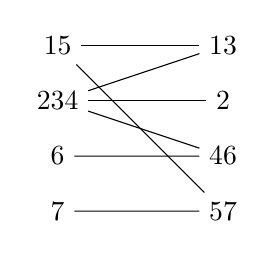
\begin{tikzpicture}[scale=.7]  
\node (1) at (-1.5, -1) {$15$};
\node (2) at (-1.5, -2) {$234$};
\node (3) at (-1.5, -3) {$6$};
\node (4) at (-1.5, -4) {$7$};
%
\node (5) at (1.5, -1) {$13$};
\node (6) at (1.5, -2) {$2$};
\node (7) at (1.5, -3) {$46$};
\node (8) at (1.5, -4) {$57$};
%
\draw[-] (1)--(5); 
\draw[-] (1)--(8);
\draw[-] (2)--(5); 
\draw[-] (2)--(6); 
\draw[-] (2)--(7); 
\draw[-] (3)--(7);
\draw[-] (4)--(8);
%
\end{tikzpicture}
$\quad$
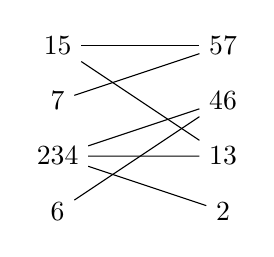
\begin{tikzpicture}[scale=.7]  
\node (1) at (-1.5, -1) {$15$};
\node (2) at (-1.5, -2) {$7$};
\node (3) at (-1.5, -3) {$234$};
\node (4) at (-1.5, -4) {$6$};
%
\node (5) at (1.5, -1) {$57$};
\node (6) at (1.5, -2) {$46$};
\node (7) at (1.5, -3) {$13$};
\node (8) at (1.5, -4) {$2$};
%
\draw[-] (1)--(5); 
\draw[-] (1)--(7);
\draw[-] (2)--(5); 
\draw[-] (3)--(6); 
\draw[-] (3)--(7); 
\draw[-] (3)--(8); 
\draw[-] (4)--(6);
%
\end{tikzpicture}
\end{center}
Here are two examples paths providing order information.
\begin{align*}
	7 <_L 234 \text{ as } 7 \xrightarrow{7} 57 \xrightarrow{5} 15 \xrightarrow{1=I_*} 13 \xrightarrow{3} 234\\
	57 <_R 46 \text{ as } 57 \xrightarrow{5} 15 \xrightarrow{1=I_*} 13 \xrightarrow{3} 234 \xrightarrow{4} 46
\end{align*}
\end{example}


This order far from being arbitrary provides the unique way to order an essential complementary partition pair into an ordered partition pair of $\triangle$, as we shall demonstrate next.

First we need a geometrical lemma. \Kurt{notation clash...}
\begin{proposition}
    The paths between adjacents vertices of $P_L$ or $P_R$ are in bijection with the minimal $(I,J)$-pairs.
\end{proposition}

\begin{proof}
    By \cref{p:minimal-IJ-pairs}, it suffices to show that the paths between adjacent vertices of $P_L$ are in bijection with the solutions of the system of equations of the form $(\rho^1,\sigma^2)$. 
    To ease notation let us write $\rho$ for $\rho^1$ and $\sigma$ for $\sigma^1$. 
    Suppose that $\rho$ is obtained from $\sigma$ by merging the two blocks $\sigma_a$ and $\sigma_b$. 
    The two equations $\langle \vec \sigma_a, x \rangle =0$ and $\langle \vec \sigma_b, x \rangle =0$ now become $\langle \vec \sigma_a + \vec \sigma_b, x \rangle =0$; nothing else changes in the system. 
    Since the solution to the system $(\sigma^1,\sigma^2)$ was $x=0$, now the solution is of dimension $1$, and it is given precisely by the path between $a$ and $b$ in $G(P)$.
    Such a path is given by an alternating sequence of vertices and edges $\sigma_1:=\sigma_a, e_1, \sigma_2, e_2, \ldots, e_{k-1}, \sigma_k:=\sigma_b$. 
    Every edge $e_i \in \{1,\ldots, n\}$ is by definition the intersection $\sigma_{i} \cap \sigma_{i+1}$; thus it is the only common non-zero coordinate between $\vec \sigma_{i}$ and $\vec \sigma_{i+1}$.
    Thus the path encodes the series of equations $x_{e_1}+x_{e_{k-1}}=0$, $x_{e_1}+x_{e_2}=0$, $x_{e_2}+x_{e_3}=0$, $\ldots$, $x_{e_{k-2}}+x_{e_{k-1}}=0$. 
    Thus, $x_{e_1}=1$, $x_{e_2}=-1$, $x_{e_3}=1$, $\ldots$, $x_{e_{k-2}}=1$, $x_{e_{k-1}}=-1$ is a basis of one-dimensional space of solutions, and it gives the corresponding minimal $(I,J)$-pair. 
\end{proof}

\begin{lemma} 
\label{o well defined}
The function $o:\EC \to \OP$ that orders an essential complementary pair is well defined.
\end{lemma}

\begin{proof}
Let $P=(\sigma,\tau) = (\bigcup_{l\in L}\sigma_l,\bigcup_{r\in R} \tau_r) \in \EC$ and consider $o(P)$. 
We first show that every $(I,J)$-condition, for $(I,J) \in D(n)$, which corresponds to a path between vertices is satisfied. 
In particular, this statement will be true for minimal $(I,J)$-pairs, which will be enough in virtue of \cref{p:minimal}. 
Suppose $I,J$ corresponds to a path between two vertices on the left, i.e.
\begin{align*}
    \sigma_l = \sigma_{l_1} \xrightarrow{i_1} \tau_{r_1}\xrightarrow{j_1} \sigma_{l_2} \xrightarrow{i_2}... \xrightarrow{i_{k}} \tau_{r_{k-1}} \xrightarrow{j_k} \sigma_{l_k}= \sigma_{l'}
\end{align*}
By construction we have that $I = \{i_1,...,i_k\},J=\{j_1,...,j_k\} \in D(n)$ (note we are ordering $I$ and $J$ by the path, so it is not necessarily the case that $\min I = i_1$). 
Furthermore, each sub partition of $\tau$ either contains a single element of $I$ and a single element of $J$, or it contains no elements of $I$ and no elements of $J$. 
As such for any ordering of the sub-partitions of $\tau$ we have that \Kurt{Could use [-] notation, but feels clearer to write out?}
\begin{align*}
    \forall m, \bigg|\bigcup_{1\leq k \leq m} \tau_{k} \cap I \bigg| = \bigg|\bigcup_{1\leq k \leq m} \tau_{k} \cap J \bigg|
\end{align*}
Hence in order for this $D(n)$ condition to be satisfied it must be the case that for some ordering of the sub-partitions of $\sigma$ we have
\begin{align*}
    \exists m, \bigg| \bigcup_{1\leq k \leq m} \sigma_k \cap I \bigg| > \bigg|\bigcup_{1\leq k \leq m} \sigma_k \cap J \bigg|
\end{align*}
Every sub-partition of $\sigma$ excluding $\sigma_l$ and $\sigma_{l'}$ either contains no elements of both $I$ and $J$, or it contains a single element of $I$ and a single element of $J$. 
So the only way for the condition to be satisfied is for $\sigma_l$ to come before $\sigma_{l'}$, which is precisely what is required by the total order.

If $I,J$ correspond to a path between two vertices on the right,
\begin{align*}
    \tau_r = \tau_{r_1} \xrightarrow{j_1} \sigma_{l_1}\xrightarrow{i_1} \tau_{r_2} \xrightarrow{j_2}... \xrightarrow{j_{k}} \sigma_{l_{k-1}} \xrightarrow{1_k} \tau_{r_k}=\tau_{r'}
\end{align*}
then a similar chain of logic implies we must have an ordering of the sub-partitions of $\tau$ such that
\begin{align*}
    \exists m, |\bigcup_{1\leq k \leq m}\tau_k \cap I| < |\bigcup_{1\leq k \leq m} \tau_k \cap J|
\end{align*}
and this can only happen if $\tau_r$ comes before $\tau_{r'}$.
\end{proof}

\begin{rem}
    It would be interesting to know if there is a geometrical interpretation of the paths that are not between adjacent vertices. 
    
\end{rem}

To complete the proof of \cref{thm:facets}, it remains to show that both $u:\OP \to \EC$ and $o:\EC\to \OP$ are injective, with the other function being their inverse.

\begin{proof}[{Proof of \cref{thm:facets}}]
The forgetful function $u$ is clearly the inverse to $o$ as forgetting any assigned order will clearly return the original essential complementary partition pair. 
The ordering function $o$ is the inverse to $u$ as it returns the sole ordering of the sub-partitions which is compatible with the $D(n)$ conditions.
\end{proof}

So the results of this section provide us with the follow characterisation of facets of the $\LAD$ diagonal.
\begin{proposition}
The facets of the $\LAD$ diagonal are ordered essential complementary partitions in which the minimal element of each path is traversed left to right.
\end{proposition}

The bijection $\theta:\SUD \to \LAD$ may be used to characterise the facets of $\SUD$ as being ordered essential complementary partitions. The bijective ordering function $o':\EC\to \SUD$ is identical to \cref{const:total order on blocks of EC}, but orients each path so that the maximal element points right to left, i.e. 
\begin{proposition}\label{prop:SUD are ordered EC}
The facets of the $\SUD$ diagonal are ordered essential complementary partitions in which the maximal element of each path is traversed right to left.
\end{proposition}
We illustrate by example how the bijection $\theta$ immediately induces this result, and note that the result can also be obtained by simply altering the constructions of the section in the obvious manner for the $\SUD$ diagonal.
\begin{example}\label{ex:theta and path translation}
We apply the bijection $\theta:\LAD\to \SUD$ to a previously encountered element of $\LAD$, \cref{ex:ECbijection}.
\begin{center}
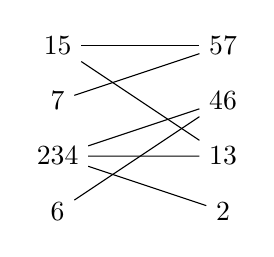
\begin{tikzpicture}[scale=.7]  
\node (1) at (-1.5, -1) {$15$};
\node (2) at (-1.5, -2) {$7$};
\node (3) at (-1.5, -3) {$234$};
\node (4) at (-1.5, -4) {$6$};
%
\node (5) at (1.5, -1) {$57$};
\node (6) at (1.5, -2) {$46$};
\node (7) at (1.5, -3) {$13$};
\node (8) at (1.5, -4) {$2$};
%
\draw[-] (1)--(5); 
\draw[-] (1)--(7);
\draw[-] (2)--(5); 
\draw[-] (3)--(6); 
\draw[-] (3)--(7); 
\draw[-] (3)--(8); 
\draw[-] (4)--(6);
%
\end{tikzpicture}
$
\xrightarrow{\theta}
$
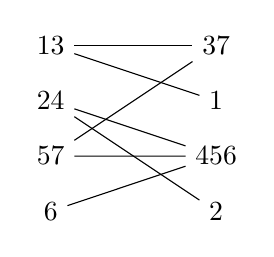
\begin{tikzpicture}[scale=.7]  
\node (1) at (-1.5, -1) {$13$};
\node (2) at (-1.5, -2) {$24$};
\node (3) at (-1.5, -3) {$57$};
\node (4) at (-1.5, -4) {$6$};
%
\node (5) at (1.5, -1) {$37$};
\node (6) at (1.5, -2) {$1$};
\node (7) at (1.5, -3) {$456$};
\node (8) at (1.5, -4) {$2$};
%
\draw[-] (1)--(5);
\draw[-] (1)--(6); 
\draw[-] (2)--(7);
\draw[-] (2)--(8);
\draw[-] (3)--(5); 
\draw[-] (3)--(7);
\draw[-] (4)--(7);
%
\end{tikzpicture}
\end{center}
Observe that the $\LA(n)$ conditions corresponding to paths, such as $( \{1,4,\},\{3,5\}) \in \LA(n)$
\begin{align*}
    57 <_R 46 \text{ as } 57 \xrightarrow{5} 15 \xrightarrow{1=I_*} 13 \xrightarrow{3} 234 \xrightarrow{4} 46
\end{align*}
are mapped to $\SU(n)$ conditions corresponding to paths, e.g. the prior $I,J$ condition maps to $( \{3,5 \},\{4,7\}) \in \SU(n)$, and
\begin{align*}
    13 <_L 24 \text{ as } 13 \xrightarrow{3} 37 \xrightarrow{7=J^*} 57 \xrightarrow{5} 456 \xrightarrow{4} 24
\end{align*}

\end{example}
Note the composite $\LAD \xrightarrow{f} \EC \xrightarrow{o'} \SUD$ provides another bijection of facets, however this map is not equal to $\theta$ and is not defined on the other faces.


\subsubsection{Vertices}

We are now interested in characterizing the pairs of vertices that occur in the diagonal, that is pairs of permutations $(\sigma_1,\sigma_2) \in \triangle$. 

\begin{thm} There exists $(I,J) \in D(n)$ such that $\forall k, |\sigma_1^1\cdots\sigma_1^k \cap I| \leq |\sigma_1^1\cdots\sigma_1^k \cap J|$ and $\forall l, |\sigma_1^1\cdots\sigma_1^l \cap I| \geq |\sigma_1^1\cdots\sigma_1^l \cap J|$ (diagonal condition) if and only if $\exists (I',J')=(\{i_1,\ldots,i_m\},\{j_1,\ldots,j_m\}) \in D(m)$, $m\leq n$, such that \[\sigma_1 \cap (I'\cup J')=j_1 i_1 j_2 i_2 \cdots j_n i_n \] and \[ \sigma_2 \cap (I'\cup J') = i_2 j_1 i_3 j_2 \cdots i_n j_{n-1} i_1 j_n \ , \] where $i_1 = \min (I' \cup J')$ (fish condition). 
\end{thm}

\begin{proof}
\begin{itemize}
\item If a pair of permutations $(\sigma_1, \sigma_2) \in   \mathfrak{S}_N^2$ satisfies the fish condition, then there exist two sets $I$ and $J$ of same cardinality such that $\min(I)<\min(J)$. Denoting $\sigma_1$ and $\sigma_2$ by two words of size $N$ $\sigma_1^1 \ldots \sigma_1^N$ and $\sigma_2^1 \ldots \sigma_2^N$, then the pair $((\sigma_1, \sigma_2), (I,J))$ satisfies that for any $k$ in $\llbracket 1;N\rrbracket$, $|\sigma_1^1 \ldots \sigma_1^k \cap J| \geq |\sigma_1^1 \ldots \sigma_1^k \cap I|$ and $|\sigma_2^1 \ldots \sigma_2^k \cap I| \geq |\sigma_2^1 \ldots \sigma_2^k \cap J|$, hence the diagonal condition.
\item We will now prove the converse. Let us presume that $(\sigma_1, \sigma_2)$ is a pair of permutations satisfying the diagonal condition for a pair of sets $(I,J) \in D(n)$, minimal for the inclusion of sets.
\begin{description}
\item[Case $n=1$] 
\end{description}
If $|I|=|J|=1$, then it follows directly from the diagonal condition above that ${\sigma_1}_{| I \cup J}=j_1 i_1$ and ${\sigma_1}_{|I \cup J}=i_1 j_1$, hence the fish condition is satisfied.
\begin{description}
\item[Case $n>1$] 
\end{description}
In this case, the proof is made by absurdum 
by considering the number of "well-placed" elements of $I$ and $J$ in $\sigma_1$ and $\sigma_2$. In what follows, for any set $E$, $\sigma^{E}_i$ will stands for $(\sigma_i)_{|E}$. We write also $n_{i,k}^E$ for the number of elements of $E$ in the $k$ first letters of $\sigma_i$. The main argument in each of the small proofs below is the same: if the permutations do not satisfy the pattern described above, then it is possible to find an appropriate pair of elements $(i,j)\in I \times J$ such that $(I-i,J-j)$ satisfies the diagonal condition, hence  contradicting the minimality of $(I,J)$.

We first prove that the leftmost element of $\sigma^{I}_1$ is $i_1$. Indeed, if it is not the case, we consider $i$, the leftmost element in $\sigma^{I}_1$ and $j$ the leftmost element in $\sigma^{J}_2$. The pair $(I-i,J-j)$ is in $D(n-1)$, as $i$ is different from $i_1$. Moreover, it is clear that the diagonal condition still holds for $((\sigma_1, \sigma_2), (I,J))$. As this would contradict the minimality of $(I,J)$, the leftmost element of $\sigma^{I}_1$ is $i_1$.

We then prove that $\sigma^{I \cup J}_1$ starts by $j_1 i_1$ and that this $j_1$ is exactly the leftmost element in  $\sigma^{J}_2$. On that purpose, we suppose that either  $i_1$ is preceeded by several elements of $J$ or that the unique element of $J$ is not the leftmost one in $\sigma^{J}_2$. We then adapt the previous argument by choosing $i$ to be the leftmost element in $\sigma^{I-\{i_1\}}_1$ and $j$ the leftmost element in $\sigma^{J}_2$. The pair $(I-i,J-j)$ is in $D(n-1)$. Let us briefly explain while  the diagonal condition would still be fulfilled in this case. If $j$ is after $i_1$ in $\sigma_1$, then the difference $n_{1,k}^{J-j}-n_{1,k}^{I-i}$ is greater than $n_{1,k}^{J}-n_{1,k}^{I}$ for any $k$, hence is non negative. If $j$ is before $i_1$ in $\sigma_1$, then by hypothesis, the difference $n_{1,k}^{J-j}-n_{1,k}^{I-i}$ is:
\begin{itemize}
\item strictly positive before $i_1$ an greater than $1$ just before $i_1$
\item non negative after $i_1$
\item increase between $i_1$ and $i$
\item is equal to $n_{1,k}^{J}-n_{1,k}^{I}$ after $i$,
\end{itemize} 
hence is always non negative.
Moreover, if $i$ is after $j$ in $\sigma_2$, the diagonal condition is clearly satisfied. If $i$ is before $j$, then the difference $n_{2,k}^{I-i}-n_{1,k}^{J-j}$ is:
\begin{itemize}
\item strictly positive before $j$ an greater than $1$ just before $j$
\item is equal to $n_{2,k}^{I}-n_{1,k}^{J}$ after $j$,
\end{itemize} 
hence is always non negative. In short, if $i_1$ is preceeded by several elements of $J$ or the unique element of $J$ is not the leftmost one in $\sigma^{J}_2$, we obtain a contradiction with the minimality of $(I,J)$.

Let us now consider the biggest $k\geq 1$ such that $\sigma^{I \cup J}_1$ begins with $j_1 i_1 j_2 i_2 \ldots j_k i_k$ and $\sigma^{I \cup J}_2$ begins with $i_2 j_1 i_3 j_2\ldots i_k j_{k-1} w j_k$, where $w$ is a word with letters in $I$. We want to show that $k=n$. Let us first remark that if $k=n$, $w=i_1$. If $1\leq k<n$, then the sets $\tilde{I}=I-\{i_1, \ldots, i_k\}$ and $\tilde{J}=J-\{j_1, \ldots, j_k\}$ are non empty. Let us choose $i_{k+1}$ to be the leftmost element in $\sigma^{\tilde{I}}_1$ and $j_{k+1}$ the leftmost element in $\sigma^{\tilde{J}}_2$. We thus have $\sigma^{I \cup J}_1=j_1 i_1 j_2 i_2 \ldots j_k i_k w' i_{k+1}\ldots$, where $w'$ is in $J$ and $\sigma^{I \cup J}_2= i_2 j_1 i_3 j_2\ldots i_k j_{k-1} w j_k w'' j_{k+1}\ldots $, where $w$ and $w'$ are words with letters in $I$. The pair $(I-i_{k+1},J-j_{k+1})$ is in $D(n-1)$. Following the study as in the previous case, $\sigma_1$ always satisfies the diagonal condition for $(I-i_{k+1},J-j_{k+1})$ and $\sigma_2$ satisfies it if and only if $w \neq i$. By minimality of $(I,J)$, we then have $w=i_{k+1}$. If $k+1=n$, we are done as the only possible word in $J$ is $j_{k+1}$, hence $w'=j_{k+1}$. Otherwise, we can choose $i_{k+2}$ to be the leftmost element in $\sigma_1^{\tilde{I}-i_{k+1}}$. Using the same reasoning as above, we show that $((\sigma_1, \sigma_2),(I-i_{k+2},J-j_{k+1}))$ satisfies the diagonal condition if and only if $w'\neq j_{k+1}$. To sum up, the only possibility for $(I,J)$ to be minimal is to have $k=n$, which implies the fish condition.
\end{itemize}
\end{proof}

\begin{corollary} For any pair of permutations $(\sigma_1, \sigma_2$, there exists $(I,J) \in D(n)$ such that $((\sigma_1, \sigma_2),(I,J))$ satisfies the diagonal condition if and only if there exists $(I',J') \in E(m)$, $m<n$ such that $((\sigma_1, \sigma_2),(I',J'))$ satisfies the fish condition, with 
\begin{multline}
E(m)=\{(I,J)\in D(m)| \min(J)<\min(I-\min(I)), |\llbracket 1; k \rrbracket \cap J| > |\llbracket 1; k \rrbracket \cap I| \\ \text{ if } |\llbracket 1; k \rrbracket \cap J| \geq 2 \text{ and } I \subsetneq \llbracket 1; k \rrbracket \}
\end{multline}
\end{corollary}

\begin{proof}
It follows directly from the fish condition: if the fish condition is satisfied, as inversions of $\sigma_1$ are included in inversions of $\sigma_2$, we get $j_{k-1},j_k<i_k$ for any $k>1$.
\end{proof}

\subsection{The Saneblidze--Umble diagonal}


Here we prove that the diagonal $\OP$ admits a combinatorial description completely analogous to that of the Saneblidze--Umble diagonal \cite{SaneblidzeUmble04}. 
A direct corollary is that the two diagonals are in bijection, and moreover that the SU diagonal can be obtained from a certain choice of chambers in the fundamental hyperplane arrangements of the permutahedra, resolving a conjecture made in \cite{LA21}.
In particular, this provides an alternative proof that all known diagonals on the associahedra agree \cite{saneblidzeComparingDiagonalsAssociahedra2022}.

Given any permutation, one can canonically produce a facet of the diagonal in the following way. 

\begin{definition}
    A pair of ordered partitions $(\sigma,\tau)$ is called \emph{strong complementary} if $\sigma$ is obtained from a permutation by merging the adjacent elements which are decreasing, and $\tau$ is obtained from the same permutation by merging the adjacent elements which are increasing.
\end{definition}

An example is shown in \cref{fig:strong-complementary}.
The same argument as in \cref{l:u-well-defined} shows that the underlying pair of partitions is an essential complementary pair. 
Moreover we see directly that any path between adjacent vertices has length $2$, and that its minimum is always traversed from left to right, hence all strong complementary pairs are in $\OP$. 

\begin{figure}[h!]
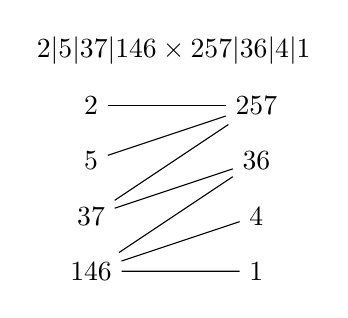
\begin{tikzpicture}[scale=.7]  
\node (p) at (0, 0) {$2|5|37|146 \times 257|36|4|1$};
\node (1) at (-1.5, -1) {$2$};
\node (2) at (-1.5, -2) {$5$};
\node (3) at (-1.5, -3) {$37$};
\node (4) at (-1.5, -4) {$146$};
%
\node (5) at (1.5, -1) {$257$};
\node (6) at (1.5, -2) {$36$};
\node (7) at (1.5, -3) {$4$};
\node (8) at (1.5, -4) {$1$};
%
\draw[-] (1)--(5); 
\draw[-] (2)--(5); 
\draw[-] (3)--(5); 
\draw[-] (3)--(6); 
\draw[-] (4)--(6); 
\draw[-] (4)--(7); 
\draw[-] (4)--(8);
%
\end{tikzpicture}
\caption{The strong complementary pair associated to the partition $2|5|7|3|6|4|1$.}
\label{fig:strong-complementary}
\end{figure}

There is a natural partial order on the facets of $\OP$. 
For two elements $x,y \in [n]$, we say that the set $\{x,y\}$ is an \emph{inversion} of a facet $(\sigma,\tau)$ if we have that $x<y$, the element $x$ appears before $y$ in $\sigma$, and the element $y$ appears before $x$ in $\tau$. 
%Visually, they appear as $\cdots | \cdots x \cdots | \cdots | \cdots y \cdots | \cdots$ in $\sigma$ and as $\cdots | \cdots y \cdots | \cdots | \cdots x \cdots | \cdots$ in $\tau$. 

\begin{definition}
    We say that two facets $(\sigma,\tau) \leq (\sigma',\tau')$ are comparable if the set of inversions of $(\sigma,\tau)$ is contained in the set of inversions of $(\sigma',\tau')$.
\end{definition}

It is immediate to see that this defines a poset.
\Guillaume{and even a lattice if a maximal and a minimal element are added?} 

\begin{proposition}
\label{p:crossings}
The set of inversions of a facet is in bijection with its set of edge crossings. 
Moreover, the set of facets with no crossings is the set of strong complementary pairs. 
\end{proposition}

\begin{proof}
    For the first part of the statement, it is clear that every inversion gives rise to a crossing. 
    For the converse, one needs to check that an anti-inversion, where $y$ appears before $x$ in $\sigma$ and $x$ appears before $y$ in $\tau$, cannot occur in a facet of $\OP$; this follows immediately from the $(I,J)$-conditions for $|I|=|J|=1$. 
    The second part of the statement follows from the fact that facets of the diagonal with no crossings are in bijection with permutations.
    As explained above, from a partition one obtains a strong complementary pair, which is in $\OP$. 
    In the other way around, given a strong complementary pair, one can read-off the partition in the associated tree, which has no crossings, by going along the edges from top to bottom, see \cref{fig:strong-complementary}.
\end{proof}


We aim now at characterizing the cover relations of this poset. 
Let $(\sigma,\tau)$ be a facet of $\OP$.
We say that a pair of adjacent blocks $\sigma_i | \sigma_{i+1}$ of $\sigma$ is \emph{admissible} if there is an element $\rho \in (\sigma_{i+1} \setminus \max\sigma_{i+1})$ such that $\rho < \min \sigma_{i}$ and $\rho < \min \gamma$ for $\gamma$ the unique path between $\sigma_i$ and $\sigma_{i+1}$. 
Such an element $\rho$ is said to be \emph{critical}. 
Let us define the \emph{left shift operator} $L$, which takes an admissible pair $\sigma_i | \sigma_{i+1}$ in $\sigma$ and creates a new ordered partition $L(\sigma)$ where the critical element $\rho$ is shifted one block to the left: we have $L(\sigma)_i := \sigma_i \cup \rho$, $L(\sigma)_{i+1} := \sigma_{i+1} \setminus \ \rho$, and $L(\sigma)_{j}:=\sigma_j$ for all $j\neq i, i+1$. 

In the same fashion, the \emph{right shift operator} $R$ sends an element $\rho \in (\tau_{i} \setminus \max\tau_{i})$ with $\rho < \min \tau_{i+1}$ and $\rho < \min \gamma$ one block to the right; the resulting ordered partition $R(\tau)$ is such that $R(\tau)_i := \tau_i \setminus \rho$ and $R(\tau)_{i+1} := \tau_{i+1} \cup \ \rho$.

\begin{definition}
    The facets of the \emph{dual SU diagonal} are the pairs or ordered partitions that can be obtained from an strong complementary pair $(\sigma,\tau)$ by iterated applications of the left shift operator $L$ on the first term $\sigma$, and iterated applications of the right shift operator $R$ on the second term $\tau$. 
\end{definition}

We shall show shortly that this definition recovers a dual of the SU diagonal on the permutahedra \cite{SaneblidzeUmble04}.

\begin{lemma}
\label{l:minima-invariance}
    Applying the left or right shift to a pair $(\sigma,\tau) \in \OP$ does not change the minima of the paths between adjacent vertices. 
\end{lemma}

\begin{proof}
We give the argument for the left shift, the one for the right one is similar. 
We observe that the paths in $(L(\sigma), \tau)$ are precisely the following: either they do not contain $\rho$, in which case they are paths of $(\sigma, \tau)$; or they do contain $\rho$, in which case they are obtained from paths in $(\sigma,\tau)$ by inserting at some place the unique path $\gamma$ between $\sigma_i$ and $\sigma_{i+1}$, or its inverse. 
Since $\rho < \min \gamma$, adding the path $\gamma$ does not change the minima of the paths in $(L(\sigma), \tau)$, with respect to the ones in $(\sigma, \tau)$.
\end{proof}

\begin{thm}
\label{t:iso-with-SU}
    The facets of the diagonal $\OP$ and the facets of the dual SU diagonal are equal. 
\end{thm}

\begin{proof}
Since we consider only the action of $L$ on the first term of the pair $(\sigma,\tau)$ and the action of $R$ on the second term, we will prove statements for $L$, the ones for $R$ are similar.

First we show that every facet of $\OP$ is a facet of the dual SU diagonal. 
Let $(\sigma,\tau)$ be a pair in $\OP$ and suppose that it satisfies the following property: for all pairs of consecutive blocks $\sigma_i | \sigma_{i+1}$ in $\sigma$, if $\min \sigma_i < \max \sigma_{i+1}$, then the unique path $\gamma$ between $\sigma_i$ and $\sigma_{i+1}$ has length $2$ and is given by $\{\min \sigma_i, \max \sigma_{i+1}\}$. 
In particular, we have $\min \sigma_i \geq \min \gamma$. 
We claim that $(\sigma,\tau)$ must be a strong complementary pair. 
To see this, suppose that $(\sigma,\tau)$ is \emph{not} a strong complementary pair; therefore by \cref{p:crossings} there exists an edge crossing. 
This implies that there is a minimal crossing, i.e. a crossing between edges adjacent to two consecutive blocks $\sigma_i | \sigma_{i+1}$. 
Since edges that are incident to a block are always in increasing order from bottom to top (this is a direct consequence of the $(I,J)$-conditions for $|I|=|J|=1$), there is a crossing between $\min \sigma_i$ and $\max \sigma_{i+1}$, which contradicts the property assumed above. 
So, there is no crossing in $(\sigma,\tau)$ and according to \cref{p:crossings}, we have that $(\sigma,\tau)$ is a strong complementary pair. 
The proof of the inclusion is now complete: if we are given a pair of facets $(\sigma,\tau)$ in $\OP$ which has at least one crossing, then there is a pair of consecutive blocks $\sigma_i | \sigma_{i+1}$ such that $\min \sigma_i < \max \sigma_{i+1}$ and $\min \sigma_i < \min \gamma$, and one can apply the inverse operator $L^{-1}$ shifting $\min \sigma_i$ to the right; and by induction we obtain a facet of the dual SU diagonal. 

Second, we show that every facet of the dual SU diagonal is in $\OP$. 
We already know that strong complementary pairs are in $\OP$. 
Thus, it suffices to prove that if a dual SU pair $(\sigma,\tau)$ is in $\OP$, then $(L(\sigma),\tau)$ is also in $\OP$. 
\cref{l:minima-invariance} shows that the minima of paths between consecutive vertices in $(L(\sigma),\tau)$ are the same as the ones in $(\sigma,\tau)$. 
Thus, all minima of paths in $(L(\sigma), \tau)$ are traversed from left to right, and we have $(L(\sigma), \tau) \in \OP$.
\end{proof}

\begin{proposition}
    \label{p:cover-relations}
    The cover relations of the poset of facets are precisely the pairs of the form $(\sigma,\tau) \prec (L(\sigma),\tau)$ and $(\sigma,\tau) \prec (\sigma,R(\tau))$ for some $L$ and $R$. 
\end{proposition}

\begin{proof} 
From the proof of \cref{t:iso-with-SU}, we know that for any facet $(\sigma,\tau) \in \OP$, we have that the pairs $(L(\sigma),\tau)$ and $(\sigma,R(\tau))$ are indeed facets of $\OP$. 

We show first that the left shift operator creates inversions, that is, for any $(\sigma, \tau) \in \OP$, we have that $(\sigma,\tau) \leq (L(\sigma),\tau)$. 
Observe that shifting a critical element to the left in $\sigma$ cannot delete any inversion: if $x<y$ and $x$ precedes $y$ in $\sigma$, then $x$ must precede $y$ also in $L(\sigma)$. 
Now, we need to show that for $x<y$, if either $y$ comes before $x$ in $\sigma$, or both $x$ and $y$ are in the same block of $\sigma$, then $y$ must come before $x$ in $\tau$. 
But this follows immediately from the $(I,J)$-condition for $I=\{x\}$ and $J=\{y\}$ defining $\OP$. 
The result then follows, since $\rho$ and $\max \sigma_{i+1}$ are in the same block of $\sigma$; thus $\max \sigma_{i+1}$ comes before $\rho$ in $\tau$ and the pair $(\rho,\max \sigma_{i+1})$ is an inversion of $(L(\sigma),\tau)$, which is not an inversion of $(\sigma,\tau)$. 

It remains to show that if $(\sigma,\tau) \leq (\sigma',\tau) \leq (L(\sigma),\tau)$, then we have either $\sigma=\sigma'$ or $\sigma'=L(\sigma)$. 
Indeed, if there is an inversion $(x,y)$ of $(L(\sigma),\tau)$ which is not an inversion of $(\sigma,\tau)$, then it must be that $x=\rho$. 
To the contrary, we have $\sigma=\sigma'$, which completes the proof. 
\end{proof}

Now we give the definition of the Saneblidze--Umble diagonal \cite{SaneblidzeUmble04}, following the description below Example $1$ in \cite{saneblidzeComparingDiagonalsAssociahedra2022}, and replace "$\max$" with "$\min$" and the symbol "$>$" with the symbol "$<$".

Let $(\sigma,\tau)$ be a pair of ordered partitions.
We say that a pair of adjacent blocks $\sigma_i | \sigma_{i+1}$ of $\sigma$ is \emph{SU admissible} if there is a non-empty subset $\rho \subset (\sigma_{i+1} \setminus \max\sigma_{i+1})$ such that $\max \rho < \min \sigma_{i}$. 
Let us define the \emph{subset left shift operator} $L^i$, which takes an SU admissible pair $\sigma_i | \sigma_{i+1}$ in $\sigma$ and creates a new ordered partition $L^i(\sigma)$ where the subset $\rho$ is shifted one block to the left: we have $L^i(\sigma)_i := \sigma_i \cup \rho$, $L^i(\sigma)_{i+1} := \sigma_{i+1} \setminus \ \rho$, and $L^i(\sigma)_{j}:=\sigma_j$ for all $j\neq i, i+1$. 
In the same fashion, the \emph{subset right shift operator} $R^i$ sends a subset $\rho \subset (\tau_{i} \setminus \max\tau_{i})$ with $\max \rho < \min \tau_{i+1}$ one block to the right; the resulting ordered partition $R^i(\tau)$ is such that $R^i(\tau)_i := \tau_i \setminus \rho$ and $R^i(\tau)_{i+1} := \tau_{i+1} \cup \ \rho$.


\begin{definition}[Dual SU diagonal, second definition]\label{def: Dual SU diagonal, second definition}
    The facets of the dual SU diagonal are the pairs of ordered partitions of the form $(L^{i_k}\cdots L^{i_1}(\sigma), R^{j_l}\cdots R^{j_1}(\tau))$ obtained from a strong complementary pair $(\sigma,\tau)$ by iterated application of subset left and right shifts operators, where moreover $i_1 > \cdots > i_k$ is decreasing and $j_1 < \cdots < j_l$ is increasing. 
\end{definition}

\begin{lemma}
\label{l:minima-invariance-subset}
    Applying the subset left or right shift to a pair $(\sigma,\tau)$ in the dual SU diagonal does not change the minima of the paths between adjacent vertices. 
\end{lemma}

\begin{proof}
    We analyse the left shift operator, the case of the right shift is similar. 
    First, we observe that any critical subset $\rho \subset L^{i_k}\cdots L^{i_1}(\sigma)_j, j \leq i_k$ satisfies $\max \rho < \min \gamma$, where $\gamma$ is the unique path between $L^{i_k}\cdots L^{i_1}(\sigma)_{j-1}=\sigma_{j-1}$ and $L^{i_k}\cdots L^{i_1}(\sigma)_j$. 
    Indeed, the path $\gamma$ is the same as the path between $\sigma_{j-1}$ and $\sigma_{j}$ in $(\sigma,\tau)$, and is equal to $\{\min \sigma_{j-1}, \max \sigma_j\}$; but since $\rho$ is critical we must have $\max \rho < \min \sigma_{j-1}=\min \gamma$. 
    The rest of the proof is the same as for \cref{l:minima-invariance}, with $\rho$ replaced by $\max \rho$. 
\end{proof}

\begin{proposition}
    The two definitions of the dual SU diagonal coincide. 
\end{proposition}

\begin{proof}
    We analyse the left shift operator, the case of the right shift is similar. 
    First, we observe that any subset left shift $L^{i}(\sigma)$ can be decomposed in a series of left shifts: since $\max \rho < \min \gamma$ by the proof of \cref{l:minima-invariance-subset}, we can first shift $\max \rho$ to the left, then $\max (\rho \setminus \max \rho)$, and so on until the entire subset $\rho$ has been shifted to the left. 
    This shows that any facet in the second definition of the dual SU diagonal is also a facet in the first definition. 

    For the reverse inclusion, we show by induction on the number of left shifts that a pair $(\sigma',\tau)$ where $\sigma'$ has been obtained by iterated left shifts can also be obtained by iterated subset left shifts, that is, can be written in the form $(L^{i_k}\cdots L^{i_1}(\sigma), \tau)$.
    The base case of a strong complementary pair is trivial. 
    Suppose that we are given a pair $(\sigma',\tau)$ where $\sigma'$ has been obtained by a sequence of $l+1$ left shifts. 
    By the induction hypothesis, the first $l$ left shifts can be rewritten as a sequence of subset left shifts, i.e. in the form $L^{i_k}\cdots L^{i_1}(\sigma)$ where $i_1 > \cdots > i_k$ are descreasing.
    Now suppose that the $(l+1)$-th left shift occurs between $L^{i_k}\cdots L^{i_1}(\sigma)_j$ and $L^{i_k}\cdots L^{i_1}(\sigma)_{j+1}$, with $j> i_k$ (otherwise, we are done!). 
    Let us denote by $\gamma$ the unique path between $L^{i_k}\cdots L^{i_1}(\sigma)_j$ and $L^{i_k}\cdots L^{i_1}(\sigma)_{j+1}$.
    By definition, we have that the critical element $\rho$ satisfies $\rho < \min \gamma$.  
    But by \cref{l:minima-invariance-subset}, this minimum is the same as the minimum of the path between $\sigma_j$ and $\sigma_{j+1}$, which is just $\min \sigma_j$. 
    Thus we have $\rho < \min \sigma_j$ (as well as $\rho < \min L^{i_k}\cdots L^{i_1}(\sigma)_j$, by criticality), and so $\rho$ can be integrated in a new or an existing subset left shift of the family $L^{i_k}\cdots L^{i_1}$, which completes the proof. 
    %also: maximum elements of each vertex never changes! so rho \neq max of its vertex
\end{proof}

One can thus interpret the left and right shift operators for singletons introduced by Saneblidze--Umble as generators of the poset of facets of the diagonal, with minimal elements the strong complementary pairs.

Now, we end with two important consequences of the preceding results. 
Consider the symmetry $s$ of the $(n-1)$-dimensional permutahedron, which consists in the reflection with respect to the hyperplane $x_1 + x_n = x_2 + x_{n-1}$. 
It sends an ordered partition $\sigma:=\sigma_1 | \ldots | \sigma_k$ to the ordered partition $s\sigma:=n-\sigma_{k}+1 | \ldots | n-\sigma_{1}+1$, where $n-\sigma_i+1$ is the set $\{n-j+1 \ | \ j \in \sigma_i\}$. 
\Kurt{This is what the next two corollaries should be i.e. altered to put max IJ =max J. Should probably combine with above.}
\begin{corollary}
\label{c:iso-with-SU}
The terms of the diagonal $\OP$ and the terms of the Saneblidze--Umble diagonal are in bijection through $(\sigma,\tau) \mapsto (s\tau,s\sigma)$
\end{corollary}

\begin{proof}
According to \cref{t:iso-with-SU}, it suffices to show that the symmetry $s$ sends the SU diagonal to the dual SU diagonal. 
\end{proof}

This allows us to prove a conjecture made in \cite[Remark 3.19]{LA21}.

\begin{corollary} \label{SU from hyperplane arrangement}
    The Saneblidze--Umble diagonal is given by the following choice of chambers in the fundamental hyperplane arrangement of the permutahedron: any vector $\vec v$ with strictly decreasing coordinates and which satisfy $\sum_{i \in I} v_i > \sum_{j \in J} v_j$ for all $I,J \subset \{1, \ldots, n\}$ such that $I \cap J = \emptyset, |I|=|J| \geq 2$ and $\max(I \cup J) \in J$ induces the Saneblidze--Umble diagonal on the $(n-1)$-dimensional standard permutahedron. 
\end{corollary}

\begin{proof}
    These orientation vectors are obtained precisely from the ones defining $\OP$ (see \cref{s:prelim}) via the symmetry described in \cref{c:iso-with-SU} above [...]. 
\end{proof}

This gives a geometric, alternative proof of the fact that all known diagonals of the associahedra agree \cite{saneblidzeComparingDiagonalsAssociahedra2022}.

\Guillaume{Thus, $(I,J)$-description for the SU diagonal...}

\Guillaume{Now we have matrix representation for free!}

\begin{example} \label{ex:shifts}
The permutation $5714632$ corresponds to the strong complementary pair $(\sigma,\tau) := 5|17|4|236 \times 57|146|3|2$. We now illustrate all possible shifts of this strong complimentary pair. The possible left shifts (indicated by their corresponding critical element, and drawn to avoid crossings) are
\begin{center}
\begin{tikzcd}
& 5|17|4|236 \times \tau \arrow[ld,"p=3"] \arrow[d,"p=1"] \arrow[rd,"p=2"]\\
5|17|34|26 \times \tau \arrow[rd,"p=1"] \arrow[d,"p=2"]&
15|7|4|236 \times \tau \arrow[rd,"p=2"] \arrow[d,"p=3"]&
5|17|24|36 \times \tau \arrow[d,"p=1"]\\
5|17|234|6 \times \tau \arrow[d,"p=1"]&
15|7|34|26 \times \tau \arrow[dl,"p=2"]&
15|17|24|36 \times \tau \\
15|7|234|6 \times \tau
\end{tikzcd}
\end{center}
The possible right shifts are simply
\begin{center}
\begin{tikzcd}
\sigma \times 57|146|3|2 \arrow[r,"p=1"] & \sigma \times 57|46|13|2 \arrow[r,"p=1"] & 57|46|3|12
\end{tikzcd}
\end{center}
As the left and right shifts can be performed independently we could combine these diagrams.
No other shifts are possible, observe for instance that we cannot perform the left shift $15|7|234|6 \times 57|46|13|2 \xrightarrow{p=2} 15|27|34|6 \times 57|46|13|2$ as the minimal path connecting $234$ and $7$ contains $1$ which is smaller than $2$ (see \cref{ex:ECbijection}). The unique way of producing $15|7|234|6 \times 57|146|3|2$ by the second definition of the SU diagonal \cref{def: Dual SU diagonal, second definition} is given by
\begin{center}
\begin{tikzcd}
5|17|4|236 \times 57|146|3|2 \arrow[r,"{p=\{2,3\}}"] & 5|17|234|6 \times 57|146|3|2 \arrow[r,"{p=\{1\}}"] & 15|7|234|6 \times 57|146|3|2
\end{tikzcd}
\end{center}
This corresponds to combining the top two arrows in the leftmost arrows of the diagram.
\end{example}

\subsection{The Saneblidze-Umble diagonal (Version 2)}

\Kurt{What do we want subscripts? superscripts? indices and/or sets?}

In this section we show that the $I,J$ description of $\SUD$, referred to as $\SUD$, is equivalent to the original description of Saneblidze-Umble diagonal \cite{SaneblidzeUmble04}, referred to as subset shift $\SUD$.
We fully detail the equalities of the top row of the following commutative diagram, (Propositions \ref{prop:subset shift to shift bijection} and \ref{prop: shift SUD and SUD are equal})
\begin{center}
\begin{tikzcd}
\text{Subset Shift $\SUD$} \arrow[r,leftrightarrow]&
\text{Shift $\SUD$} \arrow[r,leftrightarrow]&
\SUD \\
\text{Subset Shift $\LAD$} \arrow[r,dotted,leftrightarrow]&
\text{Shift $\LAD$} \arrow[r,dotted,leftrightarrow] &
\LAD \arrow[u,leftrightarrow]
\end{tikzcd}
\end{center}
, and together with the bijection $\theta:\LAD \to \SUD$ (\cref{p:IJ level bijection}) which corresponds to the vertical arrow, this proves the equivalence of the only two diagonals.
Furthermore, by duality we induce the dotted arrows of the diagram, which provides shift descriptions of the $\LAD$ diagonal ... .
\\\\
We first recall the necessary theory to describe the subset shift $\SUD$, which generates all facets by performing shifts on strong complementary partitions.
We use similar notation to the recent paper \cite{saneblidzeComparingDiagonalsAssociahedra2022}.
\begin{definition}
A pair of ordered partitions $(\sigma,\tau)$ is called \emph{strong complementary} if $\sigma$ is obtained from a permutation by merging the adjacent elements which are decreasing, and $\tau$ is obtained from the same permutation by merging the adjacent elements which are increasing.
Let $SCP$ denote the set of all strong complementary pairs.
\end{definition}

\begin{example}\label{ex:strong-complementary}
The SCP associated to the permutation $2573641$ is,
\begin{center}
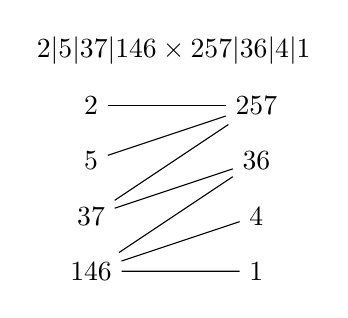
\begin{tikzpicture}[scale=.7]  
\node (p) at (0, 0) {$2|5|37|146 \times 257|36|4|1$};
\node (1) at (-1.5, -1) {$2$};
\node (2) at (-1.5, -2) {$5$};
\node (3) at (-1.5, -3) {$37$};
\node (4) at (-1.5, -4) {$146$};
%
\node (5) at (1.5, -1) {$257$};
\node (6) at (1.5, -2) {$36$};
\node (7) at (1.5, -3) {$4$};
\node (8) at (1.5, -4) {$1$};
%
\draw[-] (1)--(5); 
\draw[-] (2)--(5); 
\draw[-] (3)--(5); 
\draw[-] (3)--(6); 
\draw[-] (4)--(6); 
\draw[-] (4)--(7); 
\draw[-] (4)--(8);
%
\end{tikzpicture}
\end{center}
Observe that the permutation can be read off the graph of the SCP by a vertical down slice through the edges of the graph.
\end{example}

We make the following observations about SCPs.
Firstly, the same argument as in \cref{l:u-well-defined} shows that the underlying pair of partitions is an essential complementary pair.
Moreover, for $(\sigma,\tau)\in SCP$ we observe that 
\begin{enumerate}
    \item The unique path $\gamma$ between $\sigma_i|\sigma_{i+1}$ is $( \min \sigma_i, \max \sigma_{i+1} )$, and $\min \sigma_i< \max \sigma_{i+1}$.
    \item The unique path $\gamma$ between $\tau_i|\tau_{i+1}$ is $( \max \tau_i, \min \tau_{i+1} )$, and $\min \tau_{i+1}< \max \tau_{i}$.
\end{enumerate}
From this observation and the ordering function $o':\EC\to \SUD$ (explored in \cref{ex:theta and path translation}) it is immediate that $SCP\subset\SUD$, i.e. the maximal elements are being traversed right to left.

\begin{definition} \label{def:subset shifts}
Let $(\sigma,\tau) = (\sigma_1|...|\sigma_k,\tau_1|...|\tau_l)$ be an ordered partition pair, and let $M_i\subset (\sigma_{i}\setminus \min \sigma_{i})$ be a non-empty subset such that $\min M_i> \max \sigma_{i+1}$.
For this set we define the \emph{subset right shift operator} by
\begin{align*}
    R_{M_i}(\sigma):= \sigma_1|...|\sigma_i \setminus M_i|\sigma_i \sqcup M_i|...|\sigma_k
\end{align*}
Dually, let $M_{i+1}\subset (\tau_{i+1}\setminus \min \tau_{i+1})$  be a non-empty subset such that $\min M_{i+1}> \max \tau_{i}$.
For this set we define the \emph{subset left shift operator} by
\begin{align*}
    L_{M_{i+1}}(\tau):= \tau_1|...|\tau_i \sqcup M_{i+1}|\tau_i \setminus M_{i+1}|...|\tau_l
\end{align*}
For $l\geq 1$, let $\textbf{M} = (M_{i_1},...,M_{i_l}) \in [n]^{l}$, be such that $1\leq i_1 < i_2 ... < i_l\leq k-1$, and each of the iterated compositions $R_\mathbf{M}(\sigma) := R_{M_{i_l}}...R_{M_{i_1}}(\sigma)$ are well-defined.
Similarly, for $m\geq 1$ let $\textbf{N} = (N_{i_m},...,N_{i_1}) \in [n]^{m}$ be such that $2\leq i_1 < i_2 ... < i_m\leq k$, and each of the iterated compositions  $L_\mathbf{N}(\tau) := L_{N_{i_1}}...L_{N_{i_m}}(\tau)$ are well-defined.
We define the case $R_{\emptyset}\sigma := \sigma$ and $L_{\emptyset}\tau := \tau$. Then we denote,
\begin{align*}
    A_{\sigma}\times B_\tau:= \bigsqcup_{\mathbf{M},\mathbf{N}} \{R_\mathbf{M}(\sigma)\times L_\mathbf{N}(\tau) \}
\end{align*}
where the union is over all valid $\textbf{M},\textbf{N}$ such that the iterated operators are well-defined.
\end{definition}

See ... for an example.
Observe that the left shift operator moves elements to the left, but acts on the right ordered partition.
Dually, the right shift operator moves elements to the right but acts on the left ordered partition.
We have departed from the notation of \cite{saneblidzeComparingDiagonalsAssociahedra2022} in two ways.
Firstly we have reversed the indexing of the left shift operator, and secondly we have omitted the case $M=\emptyset$ whose corresponding operator was the identity. 
As we have omitted the case $M=\emptyset$, we have altered our indexing set from $\{1,2,...,d\}$ to the increasing sequence $i_1<...<i_d$. \Kurt{better...}
\begin{proposition}[Theorem \cite{SaneblidzeUmble04}, Restated in \cite{saneblidzeComparingDiagonalsAssociahedra2022}]
The subset-shift $SU$ diagonal is generated by all valid subset-shifts of SCPs,
\begin{align*}
    \SUD = \bigsqcup_{(\sigma,\tau) \in SCP} A_\sigma \times B_\tau
\end{align*}

\end{proposition}


We now make an interesting observation, whose proof is key to an equivalent definition of the $\SUD$ diagonal. 
\begin{lemma} \label{lem:SU subset conserves maximal element of paths}
The $\SU$ subset shift operators conserve the maximal element of paths.
In particular, given an $SCP$ $(\sigma,\tau)$ and a valid shift of it $(R_{\mathbf{M}}(\sigma),L_{\mathbf{N}}(\tau))$.
Let $\gamma_{i,j}$ denote the unique path between blocks $\sigma_i,\sigma_j$ (similarly $\tau_i,\tau_j$) and let $\gamma'_{i,j}$ denote the unique path between blocks $R_{\mathbf{M}}(\sigma)_i,R_{\mathbf{M}}(\sigma)_j$ (similarly $L_{\mathbf{N}}(\tau)_i ,L_{\mathbf{N}}(\tau)_j$), then $\max \gamma_{i,j} = \max \gamma'_{i,j} $.
\end{lemma}

\begin{proof}
We consider the right subset shift operator, and the left subset shift operator proceeds similarly.
We will prove the result inductively by assuming that for $(R_{\mathbf{M}}(\sigma),L_{\mathbf{N}}(\tau))$ we have $\max \gamma_{i,j} = \max \gamma'_{i,j}$, and then showing that if we apply a valid operator $R_{M_k}$ then we conserve this maximal element. 
As $(\sigma,\tau)$ is an SCP, we know the maximal element of the path connecting the blocks $\sigma_k|\sigma_{k+1}$ is $\max \sigma_{k+1}$. 
Hence, by the inductive hypothesis, we know that $\max \delta_{k,k+1} = \max \sigma_{k+1}$ where $\delta_{k,k+1} $ is the unique path connecting $R_{\mathbf{M}}(\sigma)_k$ and $R_{\mathbf{M}}(\sigma)_{k+1}$ in $(R_{\mathbf{M}}(\sigma),L_{\mathbf{N}}(\tau))$.
Furthermore, because $R_{M_k}$ is a valid operator we know that, $k$ is greater than the maximal index used by $\mathbf{M}$ so $\max \sigma_{k+1} = \max R_{\mathbf{M}}(\sigma)_{k+1}$, and that $\min M_k > \max R_{\mathbf{M}}(\sigma)_{k+1}$.
So combining these we know, 
\begin{align}\label{eq:shift subset dominates adj path}
    \min M_k > \max R_{\mathbf{M}}(\sigma)_{k+1} = \max \sigma_{k+1} = \max \delta_{k,k+1}
\end{align}
With this observation in hand, we explore how the shift operator $R_{M_k}$ effects paths. 
Let $\gamma$ be a path between two blocks on one side of $(R_{\mathbf{M}}(\sigma),L_{\mathbf{N}}(\tau))$, i.e. $R_{\mathbf{M}}(\sigma)_i \xrightarrow{\gamma} R_{\mathbf{M}}(\sigma)_j$ or $L_{\mathbf{N}}(\tau)_i \xrightarrow{\gamma} L_{\mathbf{N}}(\tau)_j$, and consider the path $\gamma'$ between the same blocks, by indices, in $(R_{M_k}R_{\mathbf{M}}(\sigma),L_{\mathbf{N}}(\tau))$.
For now, we assume the path $\gamma$ is not to/from either (or both) of the blocks $R_{\mathbf{M}}(\sigma)_k, R_{\mathbf{M}}(\sigma)_{k+1}$.
There are four cases to consider. 
\begin{enumerate}
    \item $\gamma$ does not contain an element of $M_k$.
    It is thus unaffected by the shift, so $\gamma' = \gamma$.
    \item $\gamma$ contains one element $m\in M_k$, i.e. $\gamma = \alpha m \beta$.
    Then there are two cases to consider
    \begin{enumerate}
        \item $\beta$ does not use any steps of $\delta_{k+1,k}$, in which case $\gamma' = \alpha m \delta_{k+1,k} \beta$.
        This is a path in the tree of $(R_{M_k}R_{\mathbf{M}}(\sigma),L_{\mathbf{N}}(\tau))$ with no repeated steps, as such it must be the unique minimal path. 
        (There cannot be another path as this would induce a cycle on the tree.)
        \item $\beta$ uses steps of $\delta_{k+1,k}$, in which case $\gamma' = \alpha m (\delta_{k+1,k}\setminus \beta)(\beta \setminus \delta_{k+1,k})$.
        This follows, as we know that $\beta$ must follow the path $\delta_{k,k+1}$ for some time before diverging ($\beta$ could also be a subset of $\delta_{k,k+1}$, in which case it will never diverge).
        As such, the path $(\delta_{k+1,k}\setminus \beta)$ reaches the point of divergence from $R_{\mathbf{M}}(\sigma)_{k+1}$ instead of $R_{\mathbf{M}}(\sigma)_{k}$, then the path $(\beta \setminus \delta_{k+1,k})$ completes the rest of the route unchanged.
    \end{enumerate}
    \item $\gamma$ contains two elements of $M_k$. In which case we still have $\gamma'=\gamma$ (in path elements) but $\gamma'$ will step through the $(k+1)$th block instead of $\gamma$ stepping through the $k$th block.
    
    \item $\gamma$ contains more than two elements of $M_k$. This is impossible, as $\gamma$ would not be a minimal path on a tree.
\end{enumerate}
We now consider the cases where $\gamma$ is a path to/from at least one of $(R_{\mathbf{M}}(\sigma))_k,(R_{\mathbf{M}}(\sigma))_{k+1}$.
We will use $j$ to denote any other arbitrary index.
We assume that $\gamma$ contains a single element $m\in M_k$ (as all other cases lead to contradictions or are trivially affected by the shift in similar logic to the prior).
Then $\gamma$ is altered by the shift to $\gamma'$ as follows,
\begin{itemize}
    \item if $\gamma$ connects $R_{\mathbf{M}}(\sigma)_j$ and $R_{\mathbf{M}}(\sigma)_k$, then $\gamma = \alpha m \mapsto \gamma' = \alpha m \delta_{k+1,k} $
    \item if $\gamma$ connects $R_{\mathbf{M}}(\sigma)_j$ and $R_{\mathbf{M}}(\sigma)_{k+1}$, then $\gamma = \alpha m \delta_{k,k+1} \mapsto \gamma' = \alpha m $
    \item if $\gamma$ connects $R_{\mathbf{M}}(\sigma)_k$ and $R_{\mathbf{M}}(\sigma)_{k+1}$, then $\gamma = \delta_{k,k+1}$ so this implies that $m\in \delta_{k,k+1}$, which is a contradiction as $m> \max \delta_{k,k+1}$.
\end{itemize}
Observe all (non-trivial or non-contradictory) paths $\gamma'$ contain $m>\min M_k$ and either some addition or deletion by $\delta_{k,k+1}$.
It thus follows from \cref{eq:shift subset dominates adj path} that $\max \gamma' = \max \gamma$, in each case, the maximal element will either be $m$ or in $\alpha,\beta$.
\end{proof}
The key result of the inductive proof was the chain of inequalities \cref{eq:shift subset dominates adj path}.
It turns out, if we assume the inequality holds, we can drop the assumption that $k$ is greater than the maximal index used by $\mathbf{M}$, and the assumption that $\min M_k > \max R_{\mathbf{M}}(\sigma)_{k+1}$. 
Furthermore, once we have dropped the assumption that we need to perform shifts in an increasing order, we can generate all subset shifts by chains of singleton set shifts. This motivates the following definition.
\begin{definition} \label{def:critical SU shift}
Let $(\sigma,\tau)$ be a pair of ordered partitions, and let $\rho \in (\sigma_i \setminus \min \sigma_i)$ such that $\rho>\max \sigma_{i,i+1}$, where $\sigma_{i,i+1}$ is the unique path between $\sigma_i$ and $\sigma_{i+1}$. Such an element $\rho$ is said to be \emph{critical}. 
We similarly define the critical elements of $\tau$ to be, $\rho \in (\tau_{i+1} \setminus \min\tau_{i+1})$ such that $\rho > \max \tau_{i,i+1}$. 
The right and left shift operators are defined on singleton sets, and we will denote these shift operators being applied to critical elements as $R_{\rho}$ and $L_{\rho}$.
\end{definition}

As we have assumed the necessary feature of the proof of \cref{lem:SU subset conserves maximal element of paths}, we have the immediate corollary.

\begin{corollary} \label{cor: SU shift conserves maximal element of paths}
The critical left and right shift operators conserve the maximal element of paths.
\end{corollary}
The observation that for an SCP $(\sigma,\tau)$ that $\max \sigma_{i,i+1} = \max \sigma_{i+1}$ (and $\max \tau_{i,i+1} = \max \tau_{i}$) then yields the following result.
\begin{corollary} \label{cor:the maximal element of shifts of SCPS}
Let $(\sigma',\tau')$ be generated from critical shifts of an SCP $(\sigma,\tau)$, then $\max \sigma'_{i,i+1} = \max \sigma_{i+1}$ (and $\max \tau'_{i,i+1} = \max \tau_{i}$).
\end{corollary}

\begin{definition}
The facets of the shift $\SUD$ are $SCP$s, and their image under iterated applications of critical left and right shift operators.
\end{definition}

As one might suspect given the above corollaries.

\begin{proposition}\label{prop:subset shift to shift bijection}
The subset shift, and shift definitions of the $\SUD$ diagonal coincide.
\end{proposition}

\begin{proof}
We analyse the right shift operator, the case of the left shift is similar. 
First, we observe that any subset right shift $R_{M_k}(\sigma)$ can be decomposed in a series of right shifts: since $\min M_k > \max \gamma$ by the proof of \cref{lem:SU subset conserves maximal element of paths}, we can first shift $\min M_k$ to the right, then $\min (M_k \setminus \min M_k)$, and so on until the entire subset $M_k$ has been shifted to the right. 
This shows that any facet of the subset shift $\SUD$ diagonal is also a facet in the shift $\SUD$ diagonal
\\\\
For the reverse inclusion, we proceed by induction. We are required to show that if we apply a critical right shift to $(R_{\mathbf{M}}(\sigma),L_{\mathbf{N}}(\tau))$, say $(R_{\rho}R_{\mathbf{M}}(\sigma),L_{\mathbf{N}}(\tau))$, then this can be re-expressed as a well-defined subset shift operation i.e. $(R_{\mathbf{M'}}(\sigma),L_{\mathbf{N}}(\tau))$. Suppose that prior to the critical shift that $\rho$ lives in block $l$, then we must have
\begin{align*}
    1 \leq i_1 < ... < i_j \leq l < i_{j+1} <...< i_d \leq k-1
\end{align*}
for some $j\in [d]$. If $i_j < l$, then $R_{\rho}R_{\mathbf{M}}(\sigma) = R_{M_{i_d}}...R_{\{\rho\}_{l}}R_{M_{i_j}}...R_{M_{i_1}}(\sigma)$, and we are done.
Otherwise, if $i_j = l$, let $M'_{i_j} = M_{i_j} \cup \{\rho \}$. It is clear that $R_{\rho}R_{\mathbf{M}}(\sigma) = R_{M_{i_d}}...R_{M'_{i_j}}...R_{M_{i_1}}(\sigma)$, however, we need to check that $R_{M'_{i_j}}$ is a well-defined subset operator. 
We know the subset shift operators will never move the minimal element, so $\rho > \min R_{\mathbf{M}}(\sigma)_{i_j}= \min (R_{M_{i_{j-1}}}...R_{M_{i_1}}(\sigma))_{i_j}$.
Then from \cref{cor:the maximal element of shifts of SCPS}, we know that $\rho>\max \sigma_{i_j+1} = \max (R_{M_{i_{j-1}}}...R_{M_{i_1}}(\sigma))_{i_j + 1}$, where the equality follows as $i_1<...<i_{j-1}<i_j$. This proves that $R_{M'_{i_j}}$ is well-defined, completing the inductive proof.
\end{proof}

\Kurt{Example!}

\begin{proposition} \label{prop: shift SUD and SUD are equal}
The facets of shift $\SUD$ and $\SUD$ are equal.
\end{proposition}
\begin{proof}
Once again, we prove our statements by considering solely the action of the right operator, the alterations for the left operator are similar. 
Firstly, we show that every facet of shift $\SUD$ is in  $\SUD$.
We already observed that all $SCP$s are in $\SUD$. Thus, it suffices to prove that if a $\SUD$ shift facet $(\sigma,\tau)$ is in $\SUD$, then $(R_{\rho}(\sigma),\tau)$ is also in $\SUD$. 
\cref{cor: SU shift conserves maximal element of paths} shows that the maxima of paths between consecutive vertices in $(R_{\rho}(\sigma),\tau)$ are the same as the ones in $(\sigma,\tau)$. 
Thus, all maxima of paths in $(R_{\rho}(\sigma),\tau)$ are traversed from right to left, and hence by \cref{prop:SUD are ordered EC}, we have that $(R_{\rho}(\sigma),\tau) \in \SUD$.
\\\\
Conversely, we now show that every facet of $\SUD$ is in shift $\SUD$. We know that every $SCP$ is an element of shift $\SUD$...\Kurt{From here onwards}
\\\\\\\\
Let $(\sigma,\tau)$ be a pair in $\OP$ and suppose that it satisfies the following property: for all pairs of consecutive blocks $\sigma_i | \sigma_{i+1}$ in $\sigma$, if $\min \sigma_i < \max \sigma_{i+1}$, then the unique path $\gamma$ between $\sigma_i$ and $\sigma_{i+1}$ has length $2$ and is given by $\{\min \sigma_i, \max \sigma_{i+1}\}$. 
In particular, we have $\min \sigma_i \geq \min \gamma$. 
We claim that $(\sigma,\tau)$ must be a strong complementary pair. 
To see this, suppose that $(\sigma,\tau)$ is \emph{not} a strong complementary pair; therefore by \cref{p:crossings} there exists an edge crossing. 
This implies that there is a minimal crossing, i.e. a crossing between edges adjacent to two consecutive blocks $\sigma_i | \sigma_{i+1}$. 
Since edges that are incident to a block are always in increasing order from bottom to top (this is a direct consequence of the $(I,J)$-conditions for $|I|=|J|=1$), there is a crossing between $\min \sigma_i$ and $\max \sigma_{i+1}$, which contradicts the property assumed above. 
So, there is no crossing in $(\sigma,\tau)$ and according to \cref{p:crossings}, we have that $(\sigma,\tau)$ is a strong complementary pair. 
The proof of the inclusion is now complete: if we are given a pair of facets $(\sigma,\tau)$ in $\OP$ which has at least one crossing, then there is a pair of consecutive blocks $\sigma_i | \sigma_{i+1}$ such that $\min \sigma_i < \max \sigma_{i+1}$ and $\min \sigma_i < \min \gamma$, and one can apply the inverse operator $L^{-1}$ shifting $\min \sigma_i$ to the right; and by induction we obtain a facet of the dual SU diagonal. 

\end{proof}

\begin{definition}
Let $(\sigma,\tau)$ be a pair of ordered partitions $[n]$, we say that $(i,j)$ where $i<j$ is a crossing if $i<_\sigma j$ and $j>_\tau i$.
\end{definition}
When we represent pairs of ordered partitions as bipartite graphs, then crossing produce 'crossings of edges' hence the name.

\begin{lemma}
For $(\sigma,\tau) \in \SUD$, it is an $SCP$ $\iff$ its bipartite graph has no crossings $\iff$ its adjacent blocks are connected by paths of length $2$.
\end{lemma}
\begin{proof}
From the fact that the permutation of a $SCP$ can be read off a downwards vertical slice (see \cref{ex:strong-complementary}), it is straightforward to verify that a $SCP$ satisfies both properties. We now verify that if $(\sigma,\tau)$ is not a $SCP$ then both these results are false.
\end{proof}

We now state the analogous shift definitions of $\LAD$.
These definitions are directly induced by the face poset isomorphism $\theta:\LAD \to \SUD$, and the fact that the critical shift operator steps through a facet of a facet to an adjacent facet. \Kurt{Maybe flesh this out into corollary and proof} See \cref{ex:shift translation by theta} to see the direct translation of the shift operators, but first, here are the definitions. 
\begin{definition}
subset def. \Kurt{maybe omit this one? a bit long...}
\end{definition}
\begin{definition} \label{def:critical LA shift}
Let $(\sigma,\tau)$ be a pair of ordered partitions, and let $\rho \in (\sigma_{i+1} \setminus \max \sigma_{i+1})$ such that $\rho< \min \sigma_{i,i+1}$, where $\sigma_{i,i+1}$ is the unique path between $\sigma_i$ and $\sigma_{i+1}$. Such an element $\rho$ is said to be \emph{critical}. 
We similarly define the critical elements of $\tau$ to be, $\rho \in (\tau_{i} \setminus \max\tau_{i})$ such that $\rho < \min \tau_{i,i+1}$. 
The right and left shift operators are defined on singleton sets, and we will denote these shift operators being applied to critical elements as $L_{\rho}$ and $R_{\rho}$
\end{definition}
We note the left shift operator now acts on the left ordered partition, a distinct notational improvement.
To illustrate how the $\LAD$ shift structure is induced by the bijection $\theta$, we provide the following example.

\begin{example} \label{ex:shift translation by theta}
The $SCP$s $(\sigma,\tau) := 5|17|4|236 \times 57|146|3|2$, and $(\sigma',\tau') := 13|247|5|6 \times 3|17|4|156$, are in bijection through $\theta$. Graphically this bijection has a clear symmetry,
\begin{center}
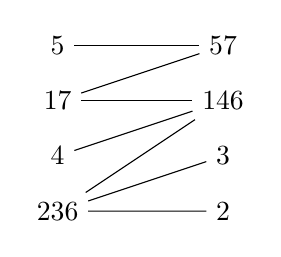
\begin{tikzpicture}[scale=.7]  
\node (1) at (-1.5, -1) {$5$};
\node (2) at (-1.5, -2) {$17$};
\node (3) at (-1.5, -3) {$4$};
\node (4) at (-1.5, -4) {$236$};
%
\node (5) at (1.5, -1) {$57$};
\node (6) at (1.5, -2) {$146$};
\node (7) at (1.5, -3) {$3$};
\node (8) at (1.5, -4) {$2$};
%
\draw[-] (1)--(5); 
\draw[-] (2)--(5); 
\draw[-] (2)--(6); 
\draw[-] (3)--(6); 
\draw[-] (4)--(6); 
\draw[-] (4)--(7); 
\draw[-] (4)--(8);
%
\end{tikzpicture}
$\xrightarrow{\theta}$
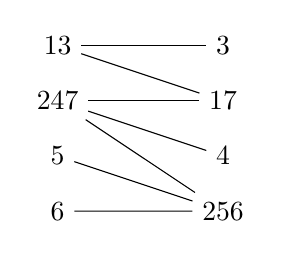
\begin{tikzpicture}[scale=.7]  
\node (1) at (-1.5, -1) {$13$};
\node (2) at (-1.5, -2) {$247$};
\node (3) at (-1.5, -3) {$5$};
\node (4) at (-1.5, -4) {$6$};
%
\node (5) at (1.5, -1) {$3$};
\node (6) at (1.5, -2) {$17$};
\node (7) at (1.5, -3) {$4$};
\node (8) at (1.5, -4) {$256$};
%
\draw[-] (1)--(5); 
\draw[-] (1)--(6); 
\draw[-] (2)--(6); 
\draw[-] (2)--(7);
\draw[-] (2)--(8); 
\draw[-] (3)--(8); 
\draw[-] (4)--(8);
%
\end{tikzpicture}
\end{center}
We now illustrate all possible $LA$ shifts of the left $SCP$ and all possible $SU$ shifts of the right $SCP$. We first display how the $LA$ left shifts act on $\sigma$, and the $SU$ left shifts act on $\tau'$. We indicate shifts by their corresponding critical element, drawing them to avoid crossings, and so they align with their dual shift under $\theta$.
\begin{center}
{\small
\begin{tikzcd}
& 5|17|4|236 \arrow[ld,"p=3"] \arrow[d,"p=1"] \arrow[rd,"p=2"]\\
5|17|34|26 \arrow[rd,"p=1"] \arrow[d,"p=2"]&
15|7|4|236  \arrow[rd,"p=2"] \arrow[d,"p=3"]&
5|17|24|36 \arrow[d,"p=1"]\\
5|17|234|6 \arrow[d,"p=1"]&
15|7|34|26  \arrow[dl,"p=2"]&
15|7|24|36  \\
15|7|234|6 
\end{tikzcd}
\begin{tikzcd}
& 3|17|4|256 \arrow[ld,red,"p=5"] \arrow[d,"p=7"] \arrow[rd,"p=6"]\\
3|17|45|26 \arrow[rd,"p=7"] \arrow[d,red,"p=6"]&
37|1|4|256 \arrow[rd,"p=6"] \arrow[d,"p=5"]&
 3|17|46|25 \arrow[d,"p=7"]\\
3|17|456|2 \arrow[d,"p=7"]&
37|1|56|24 \arrow[dl,"p=6"]&
37|1|46|25 \\
37|1|456|2
\end{tikzcd}
}
\end{center}
The possible $\LAD$ right shifts (acting on $\tau$)  are simply
\begin{center}
\begin{tikzcd}
\sigma \times 57|146|3|2 \arrow[r,"p=1"] & \sigma \times 57|46|13|2 \arrow[r,"p=1"] & 57|46|3|12
\end{tikzcd}
\end{center}
The possible $\SUD$ left shifts (acting on $\sigma'$) are 
\begin{center}
\begin{tikzcd}
13|247|5|6 \times \tau' \arrow[r,"p=7"] & \sigma \times 13|24|57|6 \arrow[r,"p=7"] & 13|24|5|67
\end{tikzcd}
\end{center}
We note that as the left and right shifts (for both diagonals) can be performed independently, we could combine these lattices into a product of lattices. \Kurt{check product correct}
No other shifts are possible, observe for instance that we cannot perform the left shift $15|7|234|6 \times 57|46|13|2 \xrightarrow{p=2} 15|27|34|6 \times 57|46|13|2$ as the minimal path connecting $234$ and $7$ contains $1$ which is smaller than $2$ (see \cref{ex:ECbijection}).
As an example of subset and critical shift bijection (\cref{prop:subset shift to shift bijection}), we observe that the unique way of producing $13|247|5|6 \times 37|1|456|2$ from subset shifts is given by
\begin{center}
\begin{tikzcd}
13|247|5|6 \times 3|17|4|256 \arrow[r,"{R_{\{5,6\}}}"] & 13|247|5|6 \times 3|17|456|2 \arrow[r,"{R_{\{7\}}}"] & 13|247|5|6 \times 37|1|456|2
\end{tikzcd}
\end{center}
This corresponds to combining the critical right shift operators of the $\SUD$ diagonal which have been indicated in red. 
\end{example}

\Kurt{Mention the LAD and SUD shifts generate the (same) facets of the hexagon in two different ways.}

We have the following equivalent characterisations of the $\LAD$ and $\SUD$ diagonals. \Kurt{Probaly in the intro somehere}
\begin{itemize}
    \item $I,J$ conditions
    \item As orderings of essential complementary partitions
    \item Subset shift
    \item Critical element shift
    \item Matrix
    \item Cubical?
\end{itemize}

\subsection{Higher algebraic consequences}

\subsubsection{Shuffle trees}

\subsection{Topological enhancement}







% !TEX root = ../Poissons.tex

\section{Tables}
\label{s:tables}

In this section we present low dimensional computations of the enumeration results obtained above and we connect them to other known combinatorial objects. 

\begin{figure}[h]
\centerline{
\begin{tabular}{r|c}
\textbf{dim} & \textbf{0}  \\
\hline
\textbf{0} & 1  
\end{tabular}
\ \ \
\begin{tabular}{r|cc}
\textbf{dim} & \textbf{0} & \textbf{1}  \\
\hline
\textbf{0} & 3 & 1 \\
\textbf{1} & 1 &  
\end{tabular}
\ \ \
\begin{tabular}{r|ccc}
\textbf{dim} & \textbf{0} & \textbf{1} & \textbf{2}  \\
\hline
\textbf{0} & 17 & 12 & 1 \\
\textbf{1} & 12 &  6 & \\
\textbf{2} & 1 &  & 
\end{tabular}
\ \ \
\begin{tabular}{r|cccc}
\textbf{dim} & \textbf{0} & \textbf{1} & \textbf{2} & \textbf{3} \\
\hline
\textbf{0} & 149 & 162 & 38 & 1 \\
\textbf{1} & 162 & 150 & 24 & \\
\textbf{2} & 38 & 24 & & \\
\textbf{3} & 1 & & &
\end{tabular}
}
\caption{Number of pairs of faces in the cellular image of the diagonal $0$, $1$, $2$ and $3$-dimensional permutahedra.}
\label{t:dim1-3}
\end{figure}

\begin{figure}[h]
\centerline{
\begin{tabular}{r|ccccc}
\textbf{dim} & \textbf{0} & \textbf{1} & \textbf{2} & \textbf{3} & \textbf{4} \\
\hline
\textbf{0} & 1809 & 2660 & 1080 & 110 & 1 \\
\textbf{1} & 2660 & 3540 & 1200 & 80 & \\
\textbf{2} & 1080 & 1200 & 270 & & \\
\textbf{3} & 110 & 80 & && \\
\textbf{4} & 1 & & & &
\end{tabular}
\ \ \
\begin{tabular}{r|cccccc}
\textbf{dim} & \textbf{0} & \textbf{1} & \textbf{2} & \textbf{3} & \textbf{4} & \textbf{5} \\
\hline
\textbf{0} & 28399 & 52635 & 30820 & 6165 & 302 & 1 \\
\textbf{1} & 52635 & 90870 & 67580 & 7785 & 240 & \\
\textbf{2} & 30820 & 47580 & 20480 & 2160 & & \\
\textbf{3} & 6165 & 7785 & 2160 & && \\
\textbf{4} & 302 & 240 & & &&\\
\textbf{5} & 1 & & & &&
\end{tabular}
}
\caption{Number of pairs of faces in the cellular image of the diagonal $4$ and $5$-dimensional permutahedra.}
\label{t:dim4-5}
\end{figure}



\begin{figure}[h]
\centerline{\begin{tabular}{c|c|rrrrrrr|l}
\textbf{Pairs $(F,G) \in \Ima\triangle_{(P,\vec v)}$} & \textbf{Polytopes} & \textbf{0} & \textbf{1} & \textbf{2} & \textbf{3} & \textbf{4} & \textbf{5} & \textbf{6} & \textbf{\cite{OEIS}} \\
\hline
& \text{Associahedra} & 1 & 2 & 6 & 22 & 91 & 408 & 1938 & \OEIS{A000139}  \\
$\dim F + \dim G = \dim P$  & \text{Multiplihedra} & 1 & 2 & 8 & 42 & 254 & 1678 & 11790 &  to appear \\
  & \text{Permutahedra} & 1 & 2 & 8 & 50 & 432 & 4802 & 65536 &  \OEIS{A007334} \\
\hline
  & \text{Associahedra} & 1 & 3 & 13 & 68 & 399 & 2530 & 16965 &  \OEIS{A000260} \\
  $\dim F=\dim G =0$ & \text{Multiplihedra} & 1 & 3 & 17 & 122 & 992 & 8721 & 80920 & to appear \\
  & \text{Permutahedra} & 1 & 3 & 17 & 149 & 1809 & 28399 & 550297 &  \OEIS{A213507} 
\end{tabular}}
\caption{Number of pairs of faces in the cellular image of the diagonal of the associahedra, multiplihedra and permutahedra of dimension $0\leq \dim P \leq 6$, induced by any good orientation vector.}
\label{table:numerology}
\end{figure}


\Guillaume{On garde?}


\subsubsection{Combinatorial formula for facets of the diagonal}

From \cref{thm:facets}, we can deduce a formula for the number of facets of the diagonal:

\begin{proposition}
The number of pairs of ordered partitions of dimension $(k,n-k)$ which correspond to facets of the diagonal is given by: 
\begin{equation}
\frac{1}{k+1}\binom{n+1}{k}(k+1)^{n-k}(n+1-k)^{k}.
\end{equation}
\end{proposition}

\begin{proof}
According to \cref{thm:facets}, pairs of ordered partitions of dimension $(k,n-k)$ which correspond to facets of the diagonal are in one-to-one correspondence with bipartite trees with $k+1$ black vertices, $n-k+1$ white vertices and $n+1$ edges labeled from $1$ to $n+1$.

We do not prove exactly here the proposition but a slightly modified version: 
Rooted bipartite trees with $k+1$ black vertices and $n-k+1$ white vertices such that:
\begin{itemize}
\item a black vertex is distinguished and called \emph{the root}
\item the $n+1$ non-root vertices are labeled,
\item every label between $1$ and $n+1$ is used exactly once.
\end{itemize}
are counted by:
\begin{equation}
\binom{n+1}{k}(k+1)^{n-k}(n+1-k)^{k}.
\end{equation}

Let us construct such a bipartite tree. 

First, there are $\binom{n+1}{k}$ ways to  choose the labels for black vertices (white vertices being labeled by the non-chosen labels). 
We denote by $\mathcal{B}$ this set of labels.

Moreover, the labeled black vertices are different from the root, hence they should have a white parent : there are $n+1-k$ ways to choose the parent of any labeled black vertex. 
We thus have  $(n+1-k)^{k}$ ways to build corollas with labeled black leaves and a white root, called bi-colored corollas (or sometimes just corollas) in the sequel.

Finally, we arrange bi-colored corollas in a rooted bipartite tree by adapting the algorithm which convert a Pr\"ufer code to a tree. 
Here what is called \emph{Pr\"ufer code} is a word of length $n-k$ over the alphabet $\mathcal{B} \cup \{\bullet\}$, where $\bullet$ stands for the non-labeled black vertex. 
Let us start with a word $c=c_1 \ldots c_{n-k} \bullet$ of length $n-k+1$ and the set $\mathcal{T}=\mathcal{S} \cup \{\bullet\}$ of $n-k+2$ bi-colored corollas augmented with the unlabeled black vertex. 
We apply Algorithm \ref{PruferWtoT}. Let us first prove it termination and correctness. The equality 
$\operatorname{length}(c)=\operatorname{Card}(\mathcal{T})-1$ is a loop invariant for the While loop: indeed at each iteration of the loop, the length of $c$ and the number of elements in $\mathcal{T}$ decrease exactly by one. It ensures the termination of the loop and the fact that $\mathcal{T}$ contains a unique element when exiting the loop. Moreover, the set of trees $\mathcal{T}$ contains at each steps exactly one unlabeled black vertex, $k$ labeled black vertices and $n-k+1$ white vertices. Finally, when adding an edge between two trees, one can only get a tree. Moreover, as the edge is added between a white root and the label of a black vertex, the obtained tree is indeed bipartite.

\begin{algorithm}[!ht]
\DontPrintSemicolon
  
  \KwInput{a word $c=c_1 \ldots c_{i}$ and a set $\mathcal{T}$ of $i$ bi-colored trees with white root and one bi-colored tree with an unlabeled black root}
  \KwOutput{a bipartite rooted tree}
  \While{$\operatorname{length}(c)>0$}{
      \tcc{loop invariant: $\operatorname{length}(c)=\operatorname{Card}(\mathcal{T})-1$, at each iteration, the length of $c$ decreases by $1$}
      t $\leftarrow \min\{a \in \mathcal{T} |$ none of the $c_i$ is a label in $a\}$ \tcp*{Here the order is given by the order on the labels of the root (as the tree with a black root does not satisfy the condition)}
      p $\leftarrow$ tree of $\mathcal{T}$ to which belongs the first letter of $c$ \tcp*{Note that it cannot be t itself}
      Remove t and p from $\mathcal{T}$ \tcp*{Decrease the cardinality of $\mathcal{T}$ by two}
      Add an edge between the root of $t$ and the first letter of $c$ and add the obtained tree to $\mathcal{T}$ \tcp*{Increase the cardinality of $\mathcal{T}$ by one}
      Remove the first letter of $c$ \tcp*{Decrease the length of $c$ by one}
  }
  {Return the unique element of $\mathcal{T}$}
  \caption{Pr\"ufer algorithm : from a word to a tree \label{PruferWtoT}}
\end{algorithm}

To prove that this algorithm defines a bijection between the pairs of Pr\"ufer code and set of bipartite rooted trees, let us give the algorithm which convert a rooted bipartite tree in such a pair in Algorithm \ref{PruferTtoW}.


\begin{algorithm}[!ht]
\DontPrintSemicolon
  
  \KwInput{a bipartite rooted tree $A$}
  \KwOutput{a word $c=c_1 \ldots c_{i}$ and a set $\mathcal{T}$ of $i$ bi-colored trees with white root, except one bi-colored tree with an unlabeled black root}
  $c \leftarrow$ empty word \tcp*{}
  $\mathcal{T} \leftarrow$ empty set \tcp*{Initialization}
  \While{$A$ has more than one vertex}{
      \tcc{At each iteration, the number of white vertices decreases by $1$}
      t $\leftarrow \min\{w \in \mathcal{T} | w$ is a white vertex whose children are leaves $\}$ \tcp*{Here the order is the one on white labels}
      $c \leftarrow c$ concatenated with label of the parent of t \tcp*{This label is a black vertex}
      Remove the edge between t and its parent: the root part goes in $A$ and the corolla in $\mathcal{T}$ \tcp*{Increase the cardinality of $\mathcal{T}$ by one}}
  {  Return the pair $(c,\mathcal{T} \cup A)$}
  \caption{Pr\"ufer algorithm : from a tree to a word \label{PruferTtoW}}
\end{algorithm}

This second algorithm terminates as the number of white vertices decreases strictly by one at each iterations. Moreover, every letter added to $c$ is the label of a black vertices, and every tree added to $\mathcal{T}$ is a bi-colored corolla or $\bullet$ (the tree with only the non-labeled black root). Finally, the cardinality of the set of bipartite trees is one more than the length of $c$. As this algorithm is the classical reverse algorithm of the first one, it ends the proof.
\BDO{Do I need to add more details ?}
\end{proof}

\begin{example} Let us apply Pr\"ufer algorithm on an example. Consider the following rooted bipartite tree on the left below, with a red root, and a redrawing of it on the right:
\begin{center}
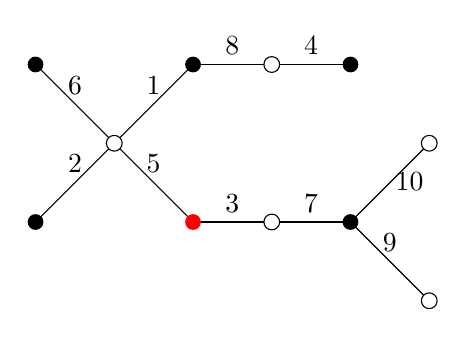
\begin{tikzpicture}
\coordinate (6) at (0,1);
\coordinate (2) at (0,-1);
\coordinate (1) at (2,1);
\coordinate (5) at (1,0);
\coordinate (8) at (3,1);
\coordinate (4) at (4,1);
\coordinate (3) at (3,-1);
\coordinate (7) at (4,-1);
\coordinate (9) at (5,-2);
\coordinate (10) at (5,0);
\coordinate (r) at (2,-1);
\draw (6)--(5) node[midway, above]{6};
\draw (2)--(5) node[midway, above]{2};
\draw (1)--(5) node[midway, above]{1};
\draw (r)--(5) node[midway, above]{5};
\draw (r)--(3) node[midway, above]{3};
\draw (3)--(7) node[midway, above]{7};
\draw (7)--(9) node[midway, above]{9};
\draw (7)--(10) node[near end, below]{10};
\draw (1)--(8) node[midway, above]{8};
\draw (8)--(4) node[midway, above]{4};
\fill (6) circle(0.1);
\fill (2) circle(0.1);
\fill (1) circle(0.1);
\fill[red] (r) circle(0.1);
\fill (4) circle(0.1);
\fill (7) circle(0.1);
\fill[draw,fill=white] (5) circle(0.1);
\fill[draw,fill=white] (3) circle(0.1);
\fill[draw,fill=white] (8) circle(0.1);
\fill[draw,fill=white] (9) circle(0.1);
\fill[draw,fill=white] (10) circle(0.1);
\end{tikzpicture}
\hspace{1cm}
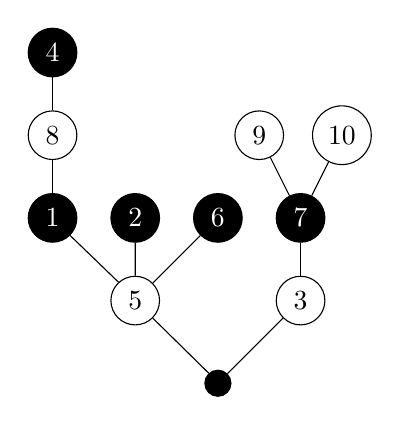
\begin{tikzpicture}[grow=up, scale=0.7,  level 1/.style={sibling distance=3cm},
    level 2/.style={sibling distance=1.5cm}]
\node[draw, circle, fill=black]{}
   child{node[draw, circle]{3}
      child{node[draw, circle, fill=black, text=white]{7}
         child{node[draw, circle]{10}
         }
         child{node[draw, circle]{9}}
      }   
   }
   child{node[draw, circle]{5}
      child{node[draw, circle, fill=black, text=white]{6}
      }   
      child{node[draw, circle, fill=black, text=white]{2}
      }   
      child{node[draw, circle, fill=black, text=white]{1}
         child{node[draw, circle]{8}
            child{node[draw, circle, fill=black, text=white]{4}}         
         }
      }   
   };
\end{tikzpicture}
\end{center}
Separating corollas with a Pr\"ufer algorithm, we get the word $1 \bullet 7 7$ and the following set of corollas:
\begin{equation*}
\left \lbrace 
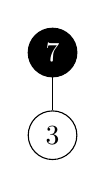
\begin{tikzpicture}[grow=up, scale=0.7, baseline=10]
\node[draw, circle]{3}
      child{node[draw, circle, fill=black, text=white]{7}};
 \end{tikzpicture},
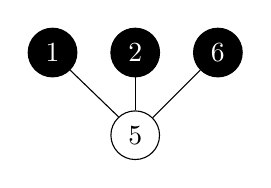
\begin{tikzpicture}[grow=up, scale=0.7, baseline=10]
\node[draw, circle]{5}
      child{node[draw, circle, fill=black, text=white]{6}
      }   
      child{node[draw, circle, fill=black, text=white]{2}
      }   
      child{node[draw, circle, fill=black, text=white]{1}
      }   ;
 \end{tikzpicture}, 
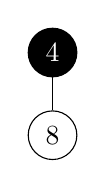
\begin{tikzpicture}[grow=up, scale=0.7, baseline=10]
\node[draw, circle]{8}
            child{node[draw, circle, fill=black, text=white]{4}} ;
 \end{tikzpicture},
 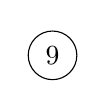
\begin{tikzpicture}[grow=up, scale=0.7, baseline=10]
\node[draw, circle]{9};
 \end{tikzpicture},
  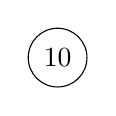
\begin{tikzpicture}[grow=up, scale=0.7, baseline=10]
\node[draw, circle]{10};
 \end{tikzpicture}
  \right \rbrace
\end{equation*}
This set of corollas can be viewed as a function $f$ from the set of labelled black vertices $\{1,2,4,6,7\}$ to the set of white vertices $\{3,5,8,9,10\}$ satisfying $f(1)=f(2)=f(6)=5$, $f(7)=3$ and $f(4)=8$.
\end{example}





\bigskip 

\emph{Acknowledgements.}    
Hugh Thomas (everything started in Montr\'eal), Sylvie Corteel for hyperplane arrangements

We would like to thank the Max Planck Institute for Mathematics in Bonn where part of this work was carried out. 
The third author was supported by the Australian Research Council Future Fellowship FT210100256.

\bibliographystyle{amsalpha}

\bibliography{Poissons}

\end{document}